% Vietnamese translation of Thesis_v3.tex (supervisor skeleton, 11 September 2026).
% Compile from the repository root with XeLaTeX:
%   latexmk -xelatex -output-directory=build archive/Thesis_v3-vi.tex
% Then copy build/Thesis_v3-vi.pdf to archive/.
%
% Distinct from archive/thesis-vi.tex, which translates the full draft
% Ha_Vien_Mastersthesis_2026.tex via archive/vi/. Chapter fragments for this
% file live in archive/vi-v3/.
%
% The class loads graphics and tikz with a hardcoded [pdftex] option, which makes
% pgf reach for pdfTeX primitives that XeTeX does not have. The drivers therefore
% have to be pinned here, before \documentclass.
\RequirePackage[pdftex,xetex]{graphicx}
\makeatletter\def\Gin@driver{xetex.def}\makeatother
\def\pgfsysdriver{pgfsys-xetex.def}

% oneside, matching Thesis_v3.tex. a4paper has to be given here: the template
% sets it with a \PassOptionsToClass placed after \documentclass.
\documentclass[english,oneside,a4paper,censored,csm,software-track-2020]{HYthesisML}

\usepackage{fontspec}
\setmainfont{lmroman10-regular.otf}[
  BoldFont=lmroman10-bold.otf,
  ItalicFont=lmroman10-italic.otf,
  BoldItalicFont=lmroman10-bolditalic.otf,
  SmallCapsFont=lmromancaps10-regular.otf]
\setsansfont{lmsans10-regular.otf}[
  BoldFont=lmsans10-bold.otf,
  ItalicFont=lmsans10-oblique.otf,
  BoldItalicFont=lmsans10-boldoblique.otf]
\setmonofont{lmmono10-regular.otf}[
  ItalicFont=lmmono10-italic.otf]

\usepackage{csquotes}

\usepackage[style=numeric,bibstyle=numeric,backend=biber,natbib=true,
            sorting=none,sortcites=true,maxbibnames=99,giveninits=true,uniquename=init]{biblatex}
\addbibresource{bibliography.bib}
\DeclareNameAlias{sortname}{family-given}
\DefineBibliographyStrings{english}{bibliography={Tài liệu tham khảo}}
\defbibheading{bibliography}[\bibname]{%
  \chapter*{#1}%
  \markboth{#1}{#1}}

\usepackage[plainpages=false]{hyperref}
\usepackage{fancyhdr}
\usepackage{longtable}
\usetikzlibrary{arrows.meta, positioning, automata, shapes.geometric, calc, fit, backgrounds}
\usepackage[section]{placeins}
\renewcommand{\topfraction}{0.9}
\renewcommand{\textfraction}{0.08}
\renewcommand{\floatpagefraction}{0.75}

\addto\captionsenglish{%
  \renewcommand{\contentsname}{Mục lục}%
  \renewcommand{\chaptername}{Chương}%
  \renewcommand{\appendixname}{Phụ lục}%
  \renewcommand{\figurename}{Hình}%
  \renewcommand{\tablename}{Bảng}%
  \renewcommand{\bibname}{Tài liệu tham khảo}%
  \renewcommand{\listfigurename}{Danh mục hình}%
  \renewcommand{\listtablename}{Danh mục bảng}%
  \renewcommand{\nomname}{Danh mục từ viết tắt}%
}

\onehalfspacing
\sloppy
\addto\extrasenglish{\frenchspacing}
\AtBeginDocument{\frenchspacing}

\newcommand{\mci}[3]{%
  \begin{tabular}[t]{@{}r@{}}%
    $#1$\\[-2pt]{\scriptsize$[#2,\,#3]$}%
  \end{tabular}}

\title{Hiệu năng, an toàn và đánh đổi kỹ thuật của Rust và C++ trong hệ thống mặt điều khiển RAN của Nokia}
\author{Ha Vien}
\date{11 tháng 9 năm 2026}
\supervisors{Prof. Keijo Heljanko, Christoph Luneburg, Petteri Kotimaa}
\examiners{Prof. Keijo Heljanko}
\keywords{Rust, C++, mặt điều khiển RAN, độ trễ đuôi, an toàn bộ nhớ, tiêm lỗi, áp dụng tăng dần}
\renewcommand{\depositeplace}{Thư viện Đại học Helsinki}
\additionalinformation{\translate{\track}}

\classification{\protect{\ \\
\  Software and its engineering $\rightarrow$ Software notations and tools $\rightarrow$ General programming languages\  \\
\  Computer systems organization $\rightarrow$ Real-time systems $\rightarrow$ Real-time system specification\\
\  Networks $\rightarrow$ Network types $\rightarrow$ Mobile networks
}}

\hypersetup{
    unicode=true,
    pdftoolbar=true,
    pdfmenubar=true,
    pdffitwindow=false,
    pdfstartview={FitH},
    pdftitle={Hiệu năng, an toàn và đánh đổi kỹ thuật của Rust và C++ trong hệ thống mặt điều khiển RAN của Nokia},
    pdfauthor={Ha Vien},
    pdfsubject={Luận văn thạc sĩ, Khoa học máy tính},
    pdfcreator={Ha Vien},
    pdfproducer={XeLaTeX},
    pdfkeywords={Rust} {C++} {mặt điều khiển RAN} {độ trễ đuôi} {an toàn bộ nhớ},
    pdfnewwindow=true,
    colorlinks=true,
    linkcolor=black,
    citecolor=black,
    filecolor=magenta,
    urlcolor=cyan
}

% Generated by bench/plot_figures.py -- do not edit by hand.
\newcommand{\ReprLoad}{28}
\newcommand{\ReprLoadAch}{28.0}
\newcommand{\ReprLoadShortfall}{0.1}
\newcommand{\SatKnee}{334}
\newcommand{\TrackingLoad}{336}
\newcommand{\NRepeats}{20}
\newcommand{\NLoadLevels}{14}
\newcommand{\NVariants}{4}
\newcommand{\NRuns}{1120}
\newcommand{\PNineNineSpread}{14}
\newcommand{\PFiftySpread}{2.9}
\newcommand{\PFiftyRange}{3}
\newcommand{\PNineNineRange}{460}
\newcommand{\PNineNineMaxCI}{2540}
\newcommand{\MaxOfferedLoad}{784}
\newcommand{\NTests}{10}
\newcommand{\MinAttainableP}{0.0000019}
\newcommand{\CorrectedFloor}{0.000019}
\newcommand{\NSignificant}{2}
\newcommand{\SmallestHolm}{0.00010}
\newcommand{\NExclZero}{4}
\newcommand{\NTailExclZero}{1}
\newcommand{\TailExclZeroRows}{p99 latency under system}
\newcommand{\RobustExclZeroRows}{p50 latency, Peak RSS and CPU utilisation under system}
\newcommand{\PFiftyDiffAbsMax}{1.6}
\newcommand{\PFiftyDiffCIMax}{3}
\newcommand{\RssLangDiffLo}{1.3}
\newcommand{\RssLangDiffHi}{1.7}
\newcommand{\RssLangCILo}{-0.5}
\newcommand{\RssLangCIHi}{1.9}
\newcommand{\CpuDiffAbsMax}{3.4}
\newcommand{\CrossAllocConsistent}{p50 latency, p99 latency, p99.9 latency, Peak RSS and CPU utilisation}
\newcommand{\CrossAllocReversed}{none}
\newcommand{\NCrossAllocReversed}{0}
\newcommand{\RssAllocDiffLo}{55.9}
\newcommand{\RssAllocDiffHi}{56.5}
\newcommand{\BudgetRepeats}{15}
\newcommand{\BudgetCoreCpp}{34.4}
\newcommand{\BudgetCoreRust}{21.3}
\newcommand{\BudgetSvcCpp}{13.52}
\newcommand{\BudgetSvcRust}{12.63}
\newcommand{\BudgetHandoffCpp}{13.49}
\newcommand{\BudgetHandoffRust}{12.61}
\newcommand{\BudgetCoreShareMax}{0.250}
\newcommand{\BudgetCoreFaster}{Rust}
\newcommand{\BudgetCoreRatio}{1.6}
\newcommand{\BudgetHandoffSlower}{C++}
\newcommand{\BudgetBoundVsCore}{101}
\newcommand{\FfiCrossing}{2.54}
\newcommand{\FfiOpRepeats}{15}
\newcommand{\FfiOpNative}{12.3}
\newcommand{\FfiOpSeam}{12.7}
\newcommand{\FfiOpDelta}{+192}
\newcommand{\FfiOpDeltaLo}{-954}
\newcommand{\FfiOpDeltaHi}{+1341}
\newcommand{\FfiOpP}{0.239}
\newcommand{\FfiOpBoundPct}{10.91}

% Generated by bench/complexity.py -- do not edit by hand.
\newcommand{\CppFuncs}{37}
\newcommand{\RustFuncs}{40}
\newcommand{\CppNloc}{511}
\newcommand{\RustNloc}{608}
\newcommand{\CppCcnTotal}{93}
\newcommand{\RustCcnTotal}{79}
\newcommand{\CppCcnMean}{2.5}
\newcommand{\RustCcnMean}{2.0}
\newcommand{\CppCcnMax}{13}
\newcommand{\RustCcnMax}{6}
\newcommand{\CppCcnMaxFn}{\texttt{worker\_loop}}
\newcommand{\RustCcnMaxFn}{\texttt{add\_drb}}
\newcommand{\CcnTotalDrop}{15}
\newcommand{\NlocRise}{19}

% Generated by bench/artefact_facts.py -- do not edit by hand.
\newcommand{\CppUeCtxBytes}{96}
\newcommand{\RustUeCtxBytes}{88}
\newcommand{\UeCtxGapBytes}{8}
\newcommand{\CppUeCtxStatePad}{3}
\newcommand{\CppUeCtxKeyEnd}{50}
\newcommand{\CppUeCtxKeyPad}{6}
\newcommand{\CppRequestBytes}{160}
\newcommand{\RustRequestBytes}{96}
\newcommand{\SignalingMsgBytes}{68}
\newcommand{\SweepUes}{5\,000}
\newcommand{\UeCtxGapTotalKB}{40}
\newcommand{\CppQueueResidentMB}{1.3}
\newcommand{\RustQueueResidentMB}{0.8}
\newcommand{\CppLineCov}{94.4}
\newcommand{\RustLineCov}{97.9}
\newcommand{\RustRegionCov}{99.1}
\newcommand{\ConfHandOps}{223}
\newcommand{\ConfGenOps}{9\,000}
\newcommand{\FfiSeamLines}{231}
\newcommand{\FfiHeaderLines}{67}
\newcommand{\FfiEntryPoints}{11}
\newcommand{\FfiUnsafeFns}{9}
\newcommand{\DeadlockTsanHits}{3}
\newcommand{\DeadlockTsanRuns}{12}
\newcommand{\FaultClasses}{14}
\newcommand{\FaultClassesPrevented}{7}
\newcommand{\FaultClassesBoundary}{7}
\newcommand{\FaultClassesUndetected}{4}
\newcommand{\LostUpdateExpected}{40\,000}
\newcommand{\LostUpdateRustHandled}{28\,714}
\newcommand{\LostUpdateRustLost}{11\,286}
\newcommand{\LostUpdateCppHandled}{27\,320}
\newcommand{\LostUpdateCppLost}{12\,680}
\newcommand{\CppTestBinaries}{6}
\newcommand{\RustTests}{27}

% Generated by bench/adoption_cost.py -- do not edit by hand.
\newcommand{\AdoptRepeats}{15}
\newcommand{\AdoptJobs}{14}
\newcommand{\BuildLibCppWall}{1.9}
\newcommand{\BuildLibRustWall}{1.2}
\newcommand{\BuildLibCppCpu}{2.6}
\newcommand{\BuildLibRustCpu}{3.9}
\newcommand{\BuildLibWallRatio}{1.7}
\newcommand{\BuildLibCpuRatio}{1.5}
\newcommand{\BuildLibWallFaster}{Rust}
\newcommand{\BuildLibCpuCheaper}{C++}
\newcommand{\BuildAllCppWall}{5.7}
\newcommand{\BuildAllRustWall}{8.1}
\newcommand{\BuildAllCppCpu}{35.9}
\newcommand{\BuildAllRustCpu}{64.8}
\newcommand{\BuildAllCpuRatio}{1.8}
\newcommand{\BuildAllFirstPartyCpu}{29.6}
\newcommand{\BuildAllFirstPartyWall}{3.8}
\newcommand{\BuildDepShareCpu}{54}
\newcommand{\BuildAllFirstPartyCpuRatio}{0.8}
\newcommand{\BuildIncCppTu}{1.2}
\newcommand{\BuildIncCppHeader}{5.8}
\newcommand{\BuildIncRust}{3.6}
\newcommand{\BuildIncTuRatio}{3.1}
\newcommand{\BuildIncHeaderRatio}{1.6}
\newcommand{\BuildConfigure}{0.91}
\newcommand{\FootTarget}{conformance\_runner}
\newcommand{\FootCppShipped}{106}
\newcommand{\FootRustShipped}{723}
\newcommand{\FootShippedRatio}{6.8}
\newcommand{\FootCppStatic}{1577}
\newcommand{\FootRustStatic}{723}
\newcommand{\FootStaticRatio}{0.5}
\newcommand{\FootCppDynamic}{106}
\newcommand{\FootRustDynamic}{269}
\newcommand{\FootDynamicRatio}{2.5}
\newcommand{\FootRustStdShare}{63}
\newcommand{\FootCppStdShare}{93}
\newcommand{\FootSharedCpp}{2531}
\newcommand{\FootSharedRust}{5295}
\newcommand{\FootStaticSmaller}{Rust}
\newcommand{\FootDynamicSmaller}{C++}
\newcommand{\FootStaticRatioAbs}{2.2}
\newcommand{\FootCppLocaleShare}{47}
\newcommand{\DepsCore}{0}
\newcommand{\DepsJemalloc}{8}
\newcommand{\DepsHarness}{17}
\newcommand{\DepsUnsafeJemalloc}{623}
\newcommand{\DepsUnsafeHarness}{1064}
\newcommand{\CoreUnsafe}{0}
\newcommand{\DepsJemallocShipping}{5}
\newcommand{\DepsJemallocBuildOnly}{3}
\newcommand{\DepsHarnessShipping}{16}
\newcommand{\DepsHarnessBuildOnly}{1}

% Generated by bench/baremetal_facts.py -- do not edit by hand.
\newcommand{\BmCores}{24}
\newcommand{\BmCounterRepeats}{10}
\newcommand{\BmCpu}{AMD EPYC 7443P}
\newcommand{\BmCpuDiffHi}{7.6}
\newcommand{\BmCpuDiffLo}{0.3}
\newcommand{\BmCpuLower}{Rust}
\newcommand{\BmCpuOneSign}{yes}
\newcommand{\BmCpuSig}{16}
\newcommand{\BmCpuTested}{16}
\newcommand{\BmCycleDelta}{15}
\newcommand{\BmCycleDeltaDir}{fewer}
\newcommand{\BmCycleDeltaP}{0.0117}
\newcommand{\BmDistro}{Ubuntu 24.04.4 LTS}
\newcommand{\BmFarTailCppHi}{228}
\newcommand{\BmFarTailCppLo}{147}
\newcommand{\BmFarTailRustHi}{115}
\newcommand{\BmFarTailRustLo}{88}
\newcommand{\BmFarTailSepHi}{96}
\newcommand{\BmFarTailSepLoad}{32}
\newcommand{\BmFarTailTopLoad}{128}
\newcommand{\BmGovernor}{performance}
\newcommand{\BmGpp}{13.3.0}
\newcommand{\BmInstrDelta}{11}
\newcommand{\BmInstrDeltaDir}{fewer}
\newcommand{\BmInstrDeltaP}{0.002}
\newcommand{\BmIsolcpus}{none}
\newcommand{\BmJeActiveCpp}{1.43}
\newcommand{\BmJeActiveDelta}{-0.64}
\newcommand{\BmJeActiveRust}{0.79}
\newcommand{\BmJeAllocatedCpp}{0.78}
\newcommand{\BmJeAllocatedDelta}{-0.16}
\newcommand{\BmJeAllocatedRust}{0.62}
\newcommand{\BmJeLiveLower}{Rust}
\newcommand{\BmJeMappedCpp}{42.82}
\newcommand{\BmJeMappedDelta}{+2.01}
\newcommand{\BmJeMappedRust}{44.83}
\newcommand{\BmJeMetaDrift}{0.5}
\newcommand{\BmJeMetadataCpp}{4.19}
\newcommand{\BmJeMetadataDelta}{+2.07}
\newcommand{\BmJeMetadataRust}{6.26}
\newcommand{\BmJeOutsideCpp}{4.0}
\newcommand{\BmJeOutsideDelta}{+3.8}
\newcommand{\BmJeOutsideRust}{7.9}
\newcommand{\BmJeResidentCpp}{11.02}
\newcommand{\BmJeResidentDelta}{-1.92}
\newcommand{\BmJeResidentRust}{9.10}
\newcommand{\BmJeRetainedCpp}{27.72}
\newcommand{\BmJeRetainedDelta}{+3.95}
\newcommand{\BmJeRetainedRust}{31.67}
\newcommand{\BmJeRssCpp}{15.08}
\newcommand{\BmJeRssDelta}{+1.74}
\newcommand{\BmJeRssRust}{16.82}
\newcommand{\BmJeRuns}{240}
\newcommand{\BmKernel}{6.17.0-23-generic}
\newcommand{\BmKneeHi}{512}
\newcommand{\BmKneeLo}{448}
\newcommand{\BmLoadHi}{128}
\newcommand{\BmLoadLevels}{8}
\newcommand{\BmLoadLo}{8}
\newcommand{\BmMetastableCv}{37}
\newcommand{\BmMetastableLoad}{512}
\newcommand{\BmMissDelta}{29}
\newcommand{\BmMissDeltaDir}{more}
\newcommand{\BmMissDeltaP}{0.002}
\newcommand{\BmNohzFull}{none}
\newcommand{\BmNumaNodes}{1}
\newcommand{\BmOverloadCv}{0.4}
\newcommand{\BmOverloadFaster}{C++}
\newcommand{\BmOverloadLoad}{640}
\newcommand{\BmOverloadThrCpp}{158}
\newcommand{\BmOverloadThrRatio}{1.64}
\newcommand{\BmOverloadThrRust}{96}
\newcommand{\BmPFiftyDiffHi}{1.1}
\newcommand{\BmPFiftyDiffLo}{0.5}
\newcommand{\BmPFiftyFaster}{Rust}
\newcommand{\BmPFiftyMedian}{74}
\newcommand{\BmPFiftySig}{14}
\newcommand{\BmPFiftyTested}{16}
\newcommand{\BmPNineNineCvMax}{2.3}
\newcommand{\BmPNineNineCvMed}{1.4}
\newcommand{\BmPNineNineMaxCI}{2.8}
\newcommand{\BmPNineNineRange}{3.6}
\newcommand{\BmPinned}{2-17}
\newcommand{\BmPoolSamplesMax}{5\,761\,198}
\newcommand{\BmPoolSamplesMin}{360\,000}
\newcommand{\BmProducers}{8}
\newcommand{\BmRepeats}{15}
\newcommand{\BmRssAllocHi}{3.2}
\newcommand{\BmRssAllocLo}{1.9}
\newcommand{\BmRssLangHi}{1.8}
\newcommand{\BmRssLangLo}{0.7}
\newcommand{\BmRssLargerEffect}{allocator}
\newcommand{\BmRssSig}{16}
\newcommand{\BmRssSpreadMax}{1.7}
\newcommand{\BmRssTested}{16}
\newcommand{\BmRuns}{480}
\newcommand{\BmRustc}{1.98}
\newcommand{\BmShards}{8}
\newcommand{\BmSmt}{off}
\newcommand{\BmSockets}{1}
\newcommand{\BmStealCores}{16}
\newcommand{\BmStealIntervals}{60}
\newcommand{\BmStealMs}{0.0}
\newcommand{\BmStealWindow}{61}
\newcommand{\BmStealWithSteal}{0}
\newcommand{\BmTrackingMax}{448}
\newcommand{\BmVirt}{none}

% Generated by bench/guest_facts.py -- do not edit by hand.
\newcommand{\GuestCores}{16}
\newcommand{\GuestCpu}{Intel(R) Xeon(R) CPU E5-2680 v4}
\newcommand{\GuestDeadlineLoad}{56}
\newcommand{\GuestDistro}{Rocky Linux 8.10 (Green Obsidian)}
\newcommand{\GuestIsolcpus}{none}
\newcommand{\GuestKernel}{7.0.2-1.el8.elrepo.x86_64}
\newcommand{\GuestLoadLevels}{14}
\newcommand{\GuestOverloadThrRatio}{1.8}
\newcommand{\GuestPFifty}{80}
\newcommand{\GuestPNineNine}{4518}
\newcommand{\GuestPNineNineMaxCI}{1480}
\newcommand{\GuestPNineNineRange}{293}
\newcommand{\GuestProducers}{7}
\newcommand{\GuestRepeats}{20}
\newcommand{\GuestRssAllocHi}{34.3}
\newcommand{\GuestRssAllocLo}{32.5}
\newcommand{\GuestRssAllocOverLang}{13}
\newcommand{\GuestRssLangHi}{3.5}
\newcommand{\GuestRssLangLo}{1.8}
\newcommand{\GuestRssLowRunOffset}{31}
\newcommand{\GuestRuns}{1120}
\newcommand{\GuestSatKnee}{336}
\newcommand{\GuestShards}{7}
\newcommand{\GuestSteal}{0}
\newcommand{\GuestThp}{always}
\newcommand{\GuestTrackingLoad}{336}
\newcommand{\GuestVirt}{kvm}


\begin{document}

\maketitle

{\singlespacing
\begin{otherlanguage}{english}
\begin{abstract}
      \noindent\textbf{Bối cảnh.}
      Phần mềm mặt điều khiển của mạng truy nhập vô tuyến (RAN) chủ yếu được viết bằng C++ vì hiệu
      năng, với cái giá đã biết về an toàn bộ nhớ và tương tranh. Rust hứa hẹn hiệu năng tương đương
      cùng an toàn tại thời điểm biên dịch, nhưng mức phù hợp cho môi trường nhạy độ trễ này vẫn chưa
      được chứng minh.

      \noindent\textbf{Mục tiêu.}
      Luận văn so sánh C++ hiện đại và Rust trên một dịch vụ Quản lý Ngữ cảnh thiết bị người dùng (UE)
      mô hình hoá theo một thành phần mặt điều khiển trạm gốc 5G thực của Nokia (gNB-CU-CP).
      So sánh thông lượng trung bình để lại bốn chiều còn mở: độ trễ đuôi, những lớp lỗi C++ mà Rust
      ngăn khi biên dịch, chi phí mô hình an toàn, và chi phí áp dụng tăng dần.

      \noindent\textbf{Phương pháp.}
      Một đặc tả độc lập ngôn ngữ được cố định trước, rồi hiện thực hai lần với thuật toán, mô hình
      tương tranh, bộ cấp phát và cấu hình biên dịch khớp nhau, và các khoảng cách bắt buộc do thành
      ngữ ngôn ngữ được ghi lại. Một khối lượng công việc tổng hợp được tăng đến quá tải, cả hai bản
      đều vượt cùng bộ kiểm thử tương đương, và phần đánh giá bổ sung tiêm lỗi cùng một nguyên mẫu
      giao diện hàm ngoại (FFI).

      \noindent\textbf{Kết quả.}
      (1)~Rust an toàn từ chối cả bảy lớp lỗi an toàn bộ nhớ và tranh chấp dữ liệu được tiêm vào tại
      thời điểm biên dịch. Ở C++ cùng bảy lớp đó biên dịch sạch. Chúng chỉ lộ ra lúc chạy, và chỉ khi
      bộ dò lỗi bắt được. (2)~Bảy lớp nữa thất bại ở cả hai ngôn ngữ. Trên hai lớp trong số đó công cụ
      C++ báo cáo những gì Rust không báo. (3)~C++ có thể gọi dịch vụ Rust qua một giao diện C mỏng.
      Toàn bộ mã \texttt{unsafe} nằm ở đó, và mọi thời gian thêm trên một cuộc gọi báo hiệu thực tối đa
      là $\FfiOpBoundPct\%$ của cuộc gọi đó. (4)~Một yêu cầu đầy đủ chỉ dành $\BudgetCoreShareMax\%$ cho
      công việc ngôn ngữ. Bàn giao giữa các luồng chiếm phần còn lại, nên đồng hồ đó không thể quy
      khoảng cách cho C++ hay Rust. Đo riêng, lõi nhanh hơn $\BudgetCoreRatio\times$ ở Rust.
      (5)~Dưới bão hoà, kiểm định ghép cặp trên trung vị đầu-cuối phân giải $\PFiftyDiffAbsMax\,\mu$s
      nghiêng về Rust. Khoảng cách đó quá nhỏ để giới hạn một hiệu ứng ngôn ngữ. Các bản Rust theo kịp
      tải đưa vào đến $\TrackingLoadRust$~kilo-thao-tác mỗi giây (kops/s), các bản C++ chỉ đến
      $\TrackingLoadCpp$. Khi cả hai đều không theo kịp, \OverloadSustainedFaster{} vẫn hoàn thành
      $\OverloadThrRatio\times$ khối lượng của \OverloadSustainedSlower{} trong \OverloadThrAgree{}
      lần lặp đan xen với cả hai bộ cấp phát.

      \noindent\textbf{Kết luận.}
      Chi phí chính khi áp dụng Rust là công sức kỹ thuật và đường cong học tập, không phải hiệu năng
      lúc chạy ở tải danh nghĩa. Lợi ích là thoát khỏi tranh chấp dữ liệu, chứ không phải mọi lỗi
      tương tranh. Một thử nghiệm ở tải danh nghĩa sẽ không lộ ra khoảng cách đó.
\end{abstract}
\end{otherlanguage}
}

\cleardoublepage
\pagenumbering{roman}
\setcounter{page}{1}
\tableofcontents

\cleardoublepage
\phantomsection
\addcontentsline{toc}{chapter}{\listfigurename}
\listoffigures

\cleardoublepage
\phantomsection
\addcontentsline{toc}{chapter}{\listtablename}
\listoftables

\cleardoublepage
\phantomsection
\addcontentsline{toc}{chapter}{\nomname}
\chapter*{\nomname}
\markboth{\nomname}{\nomname}

\noindent Mỗi từ viết tắt dưới đây cũng được viết đầy đủ tại lần dùng đầu tiên trong văn bản.

\begingroup
\singlespacing
\footnotesize
\renewcommand{\arraystretch}{1.15}
\begin{longtable}{@{}p{0.15\linewidth} p{0.79\linewidth}@{}}
\hline\hline
Viết tắt & Dạng đầy đủ \\
\hline
\endfirsthead
\hline\hline
Viết tắt & Dạng đầy đủ \\
\hline
\endhead
3GPP & 3rd Generation Partnership Project, cơ quan đặc tả các chuẩn 5G \\
ABI & Application binary interface, giao diện nhị phân ứng dụng \\
AI & Artificial intelligence, trí tuệ nhân tạo \\
AI-RAN & Kiến trúc trong đó khối lượng AI và mạng truy nhập vô tuyến dùng chung một hạ tầng gia tốc \\
API & Application programming interface, giao diện lập trình ứng dụng \\
ASN.1 & Abstract Syntax Notation One \\
CPU & Central processing unit, bộ xử lý trung tâm \\
CVE & Common Vulnerabilities and Exposures, danh mục lỗ hổng phổ biến \\
CWE & Common Weakness Enumeration, danh mục điểm yếu phổ biến \\
DPDK & Data Plane Development Kit \\
EU & European Union, Liên minh châu Âu \\
FFI & Foreign function interface, giao diện hàm ngoại \\
FIFO & First in, first out, vào trước ra trước \\
FNV-1a & Hàm băm Fowler--Noll--Vo, biến thể 1a \\
GCC & GNU Compiler Collection \\
gNB & Next-generation NodeB, trạm gốc 5G \\
gNB-CU & Đơn vị trung tâm gNB \\
gNB-CU-CP & Mặt điều khiển đơn vị trung tâm gNB: lớp hệ thống được nghiên cứu ở đây \\
gNB-CU-UP & Mặt người dùng đơn vị trung tâm gNB \\
gNB-DU & Đơn vị phân tán gNB \\
HDR & High dynamic range, dải động cao, của histogram độ trễ \\
IMT-2030 & International Mobile Telecommunications-2030, khung ITU cho 6G \\
ITU & International Telecommunication Union, Liên minh Viễn thông quốc tế \\
KPI & Key performance indicator, chỉ số hiệu năng then chốt \\
kops/s & Kilo-operations per second, kilo-thao-tác mỗi giây \\
KVM & Kernel-based Virtual Machine \\
MPSC & Multi-producer, single-consumer, nhiều tác nhân sinh, một tác nhân tiêu thụ \\
NG-RAN & Next-generation radio access network, mạng truy nhập vô tuyến thế hệ mới \\
PHY & Physical layer, tầng vật lý \\
RAII & Resource Acquisition Is Initialization \\
RAN & Radio access network, mạng truy nhập vô tuyến \\
RQ & Research question, câu hỏi nghiên cứu \\
RRC & Radio Resource Control, Điều khiển tài nguyên vô tuyến \\
RSS & Resident set size, kích thước tập trú \\
UE & User equipment, thiết bị người dùng như điện thoại hoặc modem \\
UECM & UE Context Management, phân hệ được tái hiện thực và đo ở đây \\
\hline
\end{longtable}
\endgroup

\cleardoublepage
\mainmatter

\chapter{Giới thiệu}

Mạng di động đang chuyển từ phần cứng chuyên dụng sang phần mềm trên máy chủ thông thường.
Các chức năng từng chạy trên thiết bị tích hợp theo chiều dọc, chuyên biệt cố định, nay được
tái hiện thực thành chương trình trên máy tính đa mục đích. Mạng truy nhập vô tuyến (RAN),
lâu nay là phần phụ thuộc phần cứng nhất trong ngăn xếp, cũng nằm trong xu hướng đó.

Trong 5G, trạm gốc, tên chuẩn là next-generation NodeB (gNB), được tách thành một đơn vị
trung tâm và một hoặc nhiều đơn vị phân tán. Đơn vị trung tâm lại được tách thành các chức
năng mặt điều khiển và mặt người dùng~\cite{3gpp38401,3gpp38300}. Open-RAN đẩy cùng ý tưởng
xa hơn: RAN trở thành phần mềm ảo hoá, đa nhà cung cấp, nối với nhau qua giao diện
mở~\cite{polese2023oran}. Mặt điều khiển thu được, mặt điều khiển đơn vị trung tâm gNB
(gNB-CU-CP), là một chương trình lớn, có trạng thái, tương tranh cao. Nó theo dõi mọi thiết bị
đang kết nối, mỗi thiết bị mà các chuẩn gọi là thiết bị người dùng (UE), chạy báo hiệu Điều
khiển tài nguyên vô tuyến (Radio Resource Control, RRC)~\cite{3gpp38331}, và điều phối di
động cùng chuyển giao, tất cả trong giới hạn độ trễ nghiêm ngặt.


Tải tại một site bận rộn rất cao. Một site có thể chạy hàng nghìn thủ tục quản lý kết nối và
di động mỗi giây, mỗi thủ tục phải hoàn thành trong ngân sách cỡ mili giây mà hệ thống 5G đặt
cho báo hiệu mặt điều khiển~\cite{3gpp38913}. Một mặt điều khiển triển khai có thể theo dõi
hàng triệu thiết bị hoạt động cùng lúc. Khi RAN chuyển sang triển khai đám mây, tách rời, tính
đúng đắn, độ tin cậy và thời gian của phần mềm này ngày càng quyết định chất lượng của toàn
mạng. Một sự cố hoặc một đỉnh độ trễ đuôi ở đây không phải lỗi cục bộ. Mọi thiết bị site phục
vụ đều bị ảnh hưởng~\cite{dean2013tail,barroso2017microseconds}.


Phần mềm mặt điều khiển này, hiện nay, chủ yếu được viết bằng C++. Lựa chọn đó là hợp lý:
C++ mang lại kiểm soát mức thấp, công cụ trưởng thành và hiệu năng mà hệ thống nhạy độ trễ
đòi hỏi. Nhưng hiệu năng đó đi kèm chi phí đã được biết. C++ đặt gánh nặng quản lý bộ nhớ và
tương tranh lên lập trình viên, và hàng thập kỷ kinh nghiệm cho thấy gánh nặng này thường
xuyên bị xử lý sai, sinh ra lỗi use-after-free, double-free, tranh chấp dữ liệu và các lỗi
liên quan, tốn kém để tìm, nguy hiểm khi vận hành, và chiếm phần lớn lỗ hổng bảo mật trong
thực tiễn công nghiệp~\cite{msrc2019memory,google2022android}. Rust đã nổi lên như ngôn ngữ
hệ thống đại chúng đầu tiên hứa hẹn thoát khỏi đánh đổi này: an toàn bộ nhớ và không tranh
chấp dữ liệu được thực thi lúc biên dịch trên nền tảng đã được máy
kiểm~\cite{klabnik2023rust,jung2018rustbelt}, với hiệu năng dự kiến cạnh tranh với
C++~\cite{balasubramanian2017rust}. Liệu lời hứa đó có đúng với mặt điều khiển cấp viễn thông,
nhạy độ trễ, nơi khả năng dự đoán khi quá tải quan trọng ngang tốc độ thuần, vẫn chưa được
hiểu rõ. Luận văn này, thực hiện tại Nokia, trả lời câu hỏi trực tiếp: phát triển hai bản hiện
thực tương đương về chức năng của một phân hệ RAN đại diện, một dịch vụ Quản lý Ngữ cảnh UE
mô hình hoá theo một thành phần gNB-CU-CP thật của Nokia, bằng C++ hiện đại và Rust, rồi so
sánh chúng dưới khối lượng báo hiệu tổng hợp sát thực tế.


Ba thuật ngữ lặp lại xuyên suốt. \emph{gNB-CU-CP} là phần mềm mặt điều khiển mà công trình này
xoay quanh. \emph{Quản lý Ngữ cảnh UE (UECM)} là phân hệ cụ thể được tái hiện thực và đo
lường. \emph{Độ trễ đuôi}, các phân vị p99, p99.9 và p99.99 chứ không phải trung bình, là thuộc
tính quyết định, hơn cả tốc độ trung bình, liệu hệ thống như vậy có đáp ứng hạn
chót~\cite{dean2013tail,barroso2017microseconds}.



\section{Động lực}\label{sec:motivation}
Ba xu hướng khiến phép so sánh này đúng thời điểm. Xu hướng thứ nhất là tiến hoá đám mây của
RAN. Các chức năng mặt điều khiển nay chạy trên máy chủ đa mục đích, nên phần mềm sống lâu
hơn, tương tranh cao hơn, và phải đáp ứng hạn chót mà không còn tính xác định của phần cứng
chuyên dụng. Tách rời Open-RAN biến trạm gốc thành phần mềm ảo hoá, đa nhà
cung cấp~\cite{polese2023oran}. Một hồi quy độ trễ hoặc một lỗi hỏng bộ nhớ khi đó là rủi ro
toàn mạng, và lựa chọn ngôn ngữ là một quyết định kỹ thuật.

Xu hướng thứ hai là trí tuệ nhân tạo (AI), vốn từng được mạng dùng để tự tinh chỉnh và nay
được mạng mang như một khối lượng công việc riêng~\cite{polese2026airan}. International
Mobile Telecommunications-2030 (IMT-2030), khung 6G của Liên minh Viễn thông quốc tế
(International Telecommunication Union, ITU), liệt kê vai trò thứ hai đó như một kịch bản sử
dụng~\cite{itu2023imt2030}. Kiến trúc hình thành quanh nó là AI-RAN, trong đó công việc AI và
vô tuyến dùng chung một máy chủ gia tốc~\cite{airan2026orchestrator}. Mặt điều khiển ở đó
không còn chiếm trọn máy chủ. Nó chia sẻ bộ xử lý trung tâm (CPU), bộ nhớ và cache với công
việc suy luận mà nó không lập lịch. Khi hàng xóm đó chiếm dung lượng, mặt điều khiển bão hoà
sớm hơn: nó ngừng theo kịp nhu cầu ở tải thấp hơn so với khi chạy một mình.
Chương~\ref{chapter:eval} tìm khoảng cách rộng nhất giữa hai ngôn ngữ sau điểm đó.

Xu hướng thứ ba là chuyển sang ngôn ngữ an toàn bộ nhớ. Các tổ chức phần mềm lớn báo cáo rằng
phần lớn lỗ hổng bảo mật nghiêm trọng bắt nguồn từ lỗi an toàn bộ nhớ, và việc áp dụng ngôn
ngữ an toàn bộ nhớ làm giảm chúng~\cite{msrc2019memory,google2022android,vanderstoep2025android,google2024securebydesign}.
Công trình độc lập lập luận rằng an toàn bộ nhớ nay cần yêu cầu được chuẩn hoá nếu muốn được
mua sắm~\cite{watson2025memorysafety}. Các cơ quan an ninh mạng kêu gọi rời C và C++, và Đạo
luật Cyber Resilience của Liên minh châu Âu (EU) thêm nghĩa vụ pháp lý từ tháng 9 năm 2026 và
tháng 12 năm 2027~\cite{cisa2023memorysafe,oncd2024building,eu2024cra}. Đạo luật không nêu tên
ngôn ngữ lập trình nào. Bằng chứng trực tiếp cho một mặt điều khiển RAN vẫn còn thiếu. Cung
cấp bằng chứng đó là động lực của công trình này.

\section{Bối cảnh công nghiệp}\label{sec:industrial}
Luận văn này được thực hiện tại Nokia. Công ty thuộc số ít nhà cung cấp xây, duy trì và phát
triển phần mềm RAN sản xuất từ đầu đến cuối. Năm nhà cung cấp lớn nhất chiếm 96\% doanh thu
RAN toàn cầu trong ba quý đầu năm 2025, với mức tập trung theo chỉ số Herfindahl--Hirschman
cao nhất trong mười năm~\cite{delloro2025ran3q,delloro2026ran}. Phân hệ được nghiên cứu, UECM,
được mô hình hoá theo một thành phần gNB-CU-CP thực chứ không phải ví dụ sách giáo khoa.

Trong kiến trúc của 3rd Generation Partnership Project (3GPP), gNB-CU-CP là nửa mặt điều khiển
của đơn vị trung tâm. Nó lưu RRC và quản lý vòng đời ngữ cảnh
UE~\cite{3gpp38401,3gpp38331}, dưới ngân sách cỡ mili giây mà hệ thống 5G đặt cho báo hiệu điều
khiển~\cite{3gpp38913}. Chương~\ref{chapter:background} đặt nó trong kiến trúc rộng hơn. Vì
được viết bằng C++, nó thừa hưởng hiệu năng của ngôn ngữ đó cùng các mối nguy an toàn bộ nhớ
và tương tranh. Ba xu hướng của Mục~\ref{sec:motivation} gặp nhau ở đây. Phần mềm lớp này chạy
trên mạng nhà khai thác đang vận hành. Lựa chọn ngôn ngữ là mối quan tâm sản xuất.

UECM đủ nhỏ để tái hiện thực trung thành và lý giải trọn vẹn. Nó vẫn mang những thuộc tính làm
mã mặt điều khiển khó. Hiện thực bám theo một đặc tả công khai, đã cố định, không phải mã độc
quyền, nên độc giả ngoài Nokia có thể tái lập phép so sánh.

\paragraph{Một quyết định có tầm một thế hệ.}
Một lựa chọn ngôn ngữ trong phần mềm lớp này sống lâu hơn thế hệ mà nó được đưa ra. 3GPP đã
dành Release 20 cho các nghiên cứu 6G và Release 21 cho công việc chuẩn tắc. ITU yêu cầu đề
xuất công nghệ vào đầu 2029 và nộp đặc tả vào giữa 2030~\cite{3gpp2024road6g}. Công việc đó
bao gồm di trú từ 5G và liên vận hành với 5G. Một mặt điều khiển viết hôm nay được duy trì
cùng thế hệ kế, chứ không bị loại. IMT-2030 vẫn nêu an ninh và khả năng phục hồi như nguyên
tắc thiết kế và vẫn mang kịch bản độ trễ thấp siêu tin cậy ở dạng được tăng
cường~\cite{itu2023imt2030}.

Các phép đo ở đây dùng một phân hệ thế hệ hiện tại và các yêu cầu đã công bố. Không tuyên bố
nào được đưa ra về những yêu cầu chưa được viết.

\paragraph{Một dạng lỗi cụ thể.}
Hãy xét một cơn bão di động, nhiều UE chuyển giao cùng lúc. Một ngữ cảnh UE được giải phóng
khi nhả, trong khi một thông điệp báo hiệu đang bay vẫn còn tham chiếu tới nó, là lỗi
use-after-free. Ở C++ điều đó biên dịch và có thể vượt các kiểm thử thông thường. Nó rồi có
thể làm hỏng trạng thái của một UE khác hoặc làm sập luồng xử lý dưới tương tranh cao. Cùng
lỗi đó có thể hiện ra như một đỉnh độ trễ đuôi thay vì một sự cố. Ở Rust an toàn, thiết kế
không biên dịch: sở hữu và mượn từ chối tham chiếu treo. Đó là lý do luận văn này đo cả
\emph{an toàn} (những lỗi nào được ngăn, và khi nào) lẫn \emph{khả năng dự đoán} (độ trễ đuôi
khi quá tải), chứ không chỉ thông lượng trung bình.

\section{Phát biểu bài toán}
Hai thuộc tính của miền này làm lựa chọn ngôn ngữ mang hệ quả. Thứ nhất, quản lý bộ nhớ và
tương tranh thủ công trong C++ phơi phần mềm trước các lỗi như use-after-free, double-free,
tranh chấp dữ liệu và vô hiệu hoá iterator, im lặng lúc biên dịch và tốn kém để tìm và sửa ở
quy mô viễn thông. Thứ hai, cái quyết định liệu hạn chót RAN có được đáp ứng không phải thông
lượng trung bình mà là hành vi trường hợp xấu nhất và đuôi dưới tải và quá
tải~\cite{dean2013tail}, một thuộc tính dễ hồi quy và khó đo đúng. Rust hứa loại lớp lỗi thứ
nhất tại thời điểm biên dịch trong khi tuyên bố hiệu năng cạnh tranh trên lớp thứ hai, nhưng
tuyên bố đó chủ yếu dựa trên các benchmark đa mục đích chứ không trên khối lượng viễn thông
có trạng thái, tương tranh, nhạy độ trễ.

Gộp các mạch đó lại, bài toán cụ thể mà luận văn giải quyết như sau. Các nhà cung cấp viễn
thông đang chịu áp lực ngày càng lớn, vừa kỹ thuật vừa ngày càng mang tính điều tiết, phải áp
dụng ngôn ngữ an toàn bộ nhớ, nhưng với mặt điều khiển RAN họ thiếu bằng chứng \emph{trực tiếp,
có kiểm soát} để dựa vào quyết định đó. Chưa được xác lập liệu một hiện thực Rust của một phân
hệ mặt điều khiển có trạng thái, tương tranh có thể khớp C++ hiện đại về \emph{độ trễ đuôi và
khả năng dự đoán khi quá tải} (khác với thông lượng trung bình), liệu các bảo đảm lúc biên
dịch của Rust có thực sự loại những lớp lỗi cụ thể tác động tới mã C++ sẵn có, và chi phí áp
dụng tăng dần \emph{tốn} bao nhiêu bên trong một mã nguồn C++ lớn. Bằng chứng sẵn có phần lớn
là đa mục đích và trường hợp trung
bình~\cite{balasubramanian2017rust,qin2020rust}, để lại ba câu hỏi này (khả năng dự đoán, phạm
vi lỗi được ngăn, và chi phí di trú) còn mở cho một phân hệ đại diện. Trả lời chúng trong điều
kiện có kiểm soát, tái lập được là bài toán luận văn này đặt ra để giải.

\section{Câu hỏi nghiên cứu và giả thuyết}\label{sec:rqs}
Luận văn được tổ chức quanh bốn câu hỏi nghiên cứu. Chúng đặt khả năng dự đoán độ trễ lên
trước, rồi phạm vi lỗi, rồi chi phí tài nguyên, rồi áp dụng tăng dần:

\begin{description}
  \item[RQ1] Rust và C++ hiện đại so sánh thế nào về khả năng dự đoán độ trễ (trung vị, độ trễ
        đuôi p99, p99.9 và p99.99, và cực đại) cho một khối lượng mặt điều khiển RAN dưới tải
        tăng dần và quá tải?
  \item[RQ2] Những lớp lỗi an toàn bộ nhớ và tương tranh xảy ra trong C++ nào bị loại tại thời
        điểm biên dịch trong hiện thực Rust, và các lớp còn lại được phát hiện ở giai đoạn nào
        với chi phí nào?
  \item[RQ3] Chi phí, nếu có, của mô hình an toàn Rust (kiểm biên, bản sao do sở hữu, chi phí
        trừu tượng) trên thông lượng, mức dùng CPU, và hành vi bộ nhớ là bao nhiêu?
  \item[RQ4] Những hệ quả thực tiễn (công sức, khả năng tương tác qua giao diện hàm ngoại
        (FFI), và rủi ro) của việc áp dụng Rust tăng dần trong một hệ sinh thái phần mềm RAN
        C++ sẵn có là gì?
\end{description}

Ba giả thuyết được viết ra trước mọi phép đo.
\begin{description}
  \item[H1] Với khối lượng này hai ngôn ngữ tương đương về hiệu năng dưới bão hoà, mọi khác
        biệt nếu có chỉ nằm ở đuôi xa.
  \item[H2] Rust an toàn ngăn tại thời điểm biên dịch những lớp lỗi an toàn bộ nhớ và tương
        tranh mà C++ chỉ cố bắt sau khi chương trình đã được xây.
  \item[H3] Thời gian thêm khi C++ gọi sang Rust nhỏ so với chi phí của chính các thao tác, nên
        chi phí thực của việc thêm Rust từng phần là công việc kỹ thuật, không phải tốc độ lúc
        chạy.
\end{description}
Chương~\ref{chapter:discussion} xem lại cả ba dựa trên bằng chứng.

Danh mục lỗi cho RQ2 gồm các lớp mà Rust an toàn được kỳ vọng ngăn và các lớp mà nó được kỳ
vọng không ngăn. Nghiên cứu khi đó có thể tìm nơi bảo đảm an toàn dừng lại, thay vì chỉ cho
thấy bảo đảm đó giữ.

Một nghiên cứu trước đã ước lượng biên đó từ một danh mục, không từ các chương trình được biên
dịch. Nó lấy Common Weakness Enumeration (CWE), một danh sách dài các kiểu lỗi, và đánh dấu
mỗi kiểu là kiểu mà Rust an toàn sẽ ngăn hoặc sẽ không. Nó rồi đếm các lỗ hổng thực trong 68
dự án C nguồn mở. 58.2\% các lỗ hổng được phân loại nằm ở những kiểu mà Rust an toàn gần như
đã làm không thể xảy ra~\cite{meneely2025justuserust}. Tỉ lệ đó là trường hợp tốt nhất: nó giả
định mã mới ở lại trong Rust an toàn. Một kiểu được tính là đã ngăn nếu ánh xạ nói vậy, dù
không trình biên dịch nào đã từ chối một chương trình. RQ2 hỏi cùng câu hỏi đó với các chương
trình được biên dịch và chạy. Đó là cách nó có thể nói khi nào các kiểu còn lại bị bắt, và tốn
gì để bắt chúng.

\chapter{Nền tảng: Ngôn ngữ hệ thống cho phần mềm nhạy độ trễ\label{chapter:background}}
% The class prints the chapter titles in the running head in capitals, where the
% full title of this chapter runs into the margin.
\chaptermark{Nền tảng}

\section{Hệ thống mặt điều khiển RAN và gNB-CU-CP}\label{sec:ranarch}
Mạng truy nhập vô tuyến thế hệ mới (NG-RAN) là bối cảnh của phép so sánh này. Tốc độ sự kiện
cao: UE di chuyển, và báo hiệu có thể tăng đột biến. Giới hạn trễ chặt và phải ổn định. Các
đặc tả dịch vụ và RAN 5G nêu những giới hạn đó như chỉ số hiệu năng then chốt
(KPI)~\cite{3gpp38913,3gpp22261}. Phần mềm sống lâu và tiếp tục lớn. Nhiều luồng chạy cùng lúc.
Ở đây trường hợp xấu nhất và đuôi quan trọng hơn trung bình. Đó là lý do luận văn này đo đuôi.

gNB được tách theo hai trục. Tách thứ nhất là trung tâm đối với phân tán. Một đơn vị trung tâm
(gNB-CU) lưu các tầng cao hơn của ngăn xếp. Một hoặc nhiều đơn vị phân tán (gNB-DU) lưu các
tầng thấp hơn. Những tầng đó nằm gần vô tuyến và chặt về thời gian. Tách thứ hai là mặt điều
khiển đối với mặt người dùng, bên trong đơn vị trung tâm. Nó tách chức năng mặt điều khiển
(gNB-CU-CP) khỏi chức năng mặt người dùng (gNB-CU-UP). Các phần này nói chuyện qua liên kết
chuẩn. NG đi về lõi 5G. F1 nằm giữa CU và DU. E1 nằm giữa CU-CP và
CU-UP~\cite{3gpp38401,3gpp38300,3gpp38463}. Open-RAN đẩy cùng các liên kết đó xa hơn. Mỗi phần
khi đó có thể đến từ một nhà cung cấp khác và chạy như phần mềm trên máy thông
thường~\cite{polese2023oran}. Hình~\ref{fig:ngran} đặt phân hệ được nghiên cứu ở đây, Quản lý
Ngữ cảnh UE (UECM), bên trong gNB-CU-CP. UECM sở hữu trạng thái mặt điều khiển theo từng UE.
Nó cũng xử lý báo hiệu RRC và di động. Đó là lý do tính đúng đắn và thời gian của nó đứng cho
mặt điều khiển nói chung.

% After the two paragraphs the leftover is a few points short of the TikZ plus
% caption, so [ht] defers it and [section]{placeins} ships the leftover as
% whitespace. A small enlarge keeps the figure with the section that cites it.
\enlargethispage{12pt}
\begin{figure}[!ht]
\centering
\begin{tikzpicture}[
    font=\small, >={Stealth[length=2.4mm]},
    box/.style={draw, rounded corners, minimum height=1.0cm, minimum width=1.7cm,
                align=center, fill=gray!8},
    cpbox/.style={draw, rounded corners, align=center, fill=blue!8},
    upbox/.style={draw, rounded corners, minimum width=3.1cm, minimum height=0.8cm,
                  align=center, fill=green!8},
    uecm/.style={draw, rounded corners, minimum width=2.7cm, minimum height=0.62cm,
                 fill=red!14, align=center}
  ]
  \node[box] (ue) at (0,0)   {UE};
  \node[box] (du) at (2.4,0) {gNB-DU};

  \node[font=\footnotesize\bfseries] (cpttl) at (7.2,1.7) {gNB-CU-CP};
  \node[uecm] (uecm) at (7.2,0.85) {Quản lý ngữ cảnh\\ UE};
  \node[upbox] (up) at (7.2,-0.95) {gNB-CU-UP};

  \begin{scope}[on background layer]
    \node[fit=(cpttl)(uecm), inner sep=6pt] (cp) {};
    \node[draw, dashed, rounded corners, fill=gray!3,
          fit=(cp)(up), inner sep=10pt, label={[font=\footnotesize\bfseries]above:gNB-CU}] (cu) {};
    \node[cpbox, fit=(cp), inner sep=0pt] {};
  \end{scope}

  \node[box] (core) at (11.4,0) {Lõi 5G};

  \draw[<->] (ue) -- node[above,font=\scriptsize]{Uu} (du);
  \draw[<->] (du.east)         -- node[above,font=\scriptsize]{F1} (cu.west |- du);
  \draw[<->] (cu.east |- core) -- node[above,font=\scriptsize]{NG} (core.west);
  \draw[<->] (cp.south) -- node[right,font=\scriptsize]{E1} (up.north);
\end{tikzpicture}
\caption[Phân hệ nghiên cứu nằm ở đâu trong NG-RAN 5G]{Phân hệ nghiên cứu nằm ở đâu trong
NG-RAN 5G. Quản lý Ngữ cảnh UE được tô đậm bên trong gNB-CU-CP.\label{fig:ngran}}
\end{figure}

\section{Khả năng dự đoán và hai ngôn ngữ}\label{sec:bgbrief}
Mục này nêu những gì nghiên cứu lấy làm cho trước. Độ trễ ổn định, không phải thông lượng trung
bình, là thuộc tính chính của một dịch vụ nhạy trễ. Vì vậy đại lượng cần đo là đuôi, không phải
trung bình. Đo đuôi tốt cũng định hình khung đo. Lịch gửi phải là vòng hở. Một bộ gửi vòng kín
dừng khi một tắc đang diễn ra. Nó rồi không bao giờ ghi lại độ trễ của tắc đó.

C++ cho kiểm soát mà miền cần. Nó để an toàn bộ nhớ và luồng cho lập trình viên. Bộ dò lỗi và
rà soát đứng thay cho một bảo đảm. Công việc của uỷ ban chuẩn về hồ sơ an toàn được thực thi
chưa phải một chuẩn. Nó chưa được dùng rộng. Sở hữu và mượn của Rust loại lỗi vòng đời và
aliasing tại thời điểm biên dịch. Các trait \texttt{Send} và \texttt{Sync} loại tranh chấp dữ
liệu. Tuyên bố đó hẹp hơn ``an toàn luồng''. Nó không nói gì về thứ tự khoá. Nó không nói gì về
việc một bước ghép có nguyên tử hay không. Nó không nói gì về rò rỉ. Và nó tắt ở mọi nơi chương
trình viết \texttt{unsafe}. Cả hai ngôn ngữ đều diễn đạt được cùng cấu trúc luồng. Một phép so
sánh để cấu trúc đổi theo ngôn ngữ khi đó đo cấu trúc, không đo ngôn ngữ. Hai bên gặp nhau qua
một giao diện nhị phân ứng dụng C. Đó là đường mà mọi di trú từng bước phải dùng. Đó cũng là
lý do một đường nối giữ \texttt{unsafe} mà một cuộc di trú cần.

\section{Khoảng trống nghiên cứu}\label{sec:gap}
Các mục trên dựng khoảng trống. Mặt điều khiển RAN có nhiều luồng và giới hạn trễ chặt. Độ trễ
đuôi khi tải quá lớn, không phải thông lượng trung bình, đặt chất lượng mà mạng giao. C++ cho
kiểm soát và tốc độ mà miền cần. Nhưng nó để cả lớp lỗi bộ nhớ và luồng cho phát hiện sau. Rust
hứa chặn những lớp đó tại thời điểm biên dịch mà không tốn thời gian chạy. Nó cũng cho một
đường áp dụng từng bước qua giao diện nhị phân ứng dụng (ABI) C.

Miền này không phải chưa được nghiên cứu. Khối lượng công trình trước dễ bị bỏ sót, vì gần như
không công trình nào được lập chỉ mục. Năm luận văn thạc sĩ do nhà cung cấp lưu trữ, tất cả
thực hiện tại Ericsson, đã so sánh các ngôn ngữ ứng viên cho phần mềm RAN và viễn thông. Một
bài cân chi phí lúc chạy với tốc độ con người xây được, trên C++, Rust và
Go~\cite{karlback2021ran}. Một bài hỏi liệu Rust có thể thay C trong quản lý nút
RAN~\cite{olsson2023ranmgmt}. Một bài xây bộ xử lý gói, một luồng mỗi nhân, bằng Rust async. Nó
đo bộ xử lý đó đối với chương trình Data Plane Development Kit (DPDK) mà nó
nhái~\cite{olsson2023asyncpackets}. Một bài đo độ trễ trung vị và p99 cho các bước mặt điều
khiển trên năm khung async~\cite{arvidsson2025async}. Bài cuối xây các bản C++ và Rust khớp
nhau của một bộ dịch ngược Abstract Syntax Notation One (ASN.1). Nó so sánh chúng bằng kiểm
định thống kê~\cite{emberg2023asn1}. Cả năm đều liên quan trực tiếp. Hai bài báo cáo khoảng
cách không nghiêng về Rust.

Ba trong số đó đổi ngôn ngữ cùng lúc với thời gian chạy và mô hình luồng. Một khoảng cách đo
được khi đó không thể quy cho ngôn ngữ chứ không phải khung~\cite{karlback2021ran,olsson2023asyncpackets,arvidsson2025async}.
Cỡ hiệu ứng lên tới hệ số năm. Điều đó cho thấy thời gian chạy chiếm bao nhiêu của phép đo. Hai
bài kia giữ thiết kế sát hơn với cố định. Nhưng chúng báo cáo thời gian chạy và bộ nhớ đỉnh,
không phải độ trễ đuôi dưới tải tăng~\cite{olsson2023ranmgmt,emberg2023asn1}. Bài gần nhất,
Emberg và Wadsten, đo một phép biến đổi không trạng thái. Nó không phải một phần nhiều luồng
có trạng thái. Hình~\ref{fig:gapmap} đặt năm luận văn nhà cung cấp cạnh các so sánh đa mục
đích~\cite{pereira2017energy} và các cặp phần mềm hệ thống khớp~\cite{emmerich2019drivers,suchert2023stamp}.
Mẫu hình như sau. Mỗi nhóm giữ một phần những gì một phép thử công bằng cần. Không nhóm nào giữ
hết.

Sự tập trung đó tự nó là một phần của khoảng trống. Cả năm nghiên cứu đến từ một nhà cung cấp.
Kết luận của chúng chưa bao giờ được thử đối với phần mềm, mục tiêu hay quy tắc nội bộ của một
công ty khác. Vì vậy những gì được biết về câu hỏi này là những gì khung của một công ty nói về
nó. Hồ sơ công bố phía bên kia mỏng hơn. Không có nghiên cứu về Rust trong các bài được lập chỉ
mục của nhà cung cấp chủ trì công trình này. Lập trường đã bình duyệt gần nhất từ phía đó lập
luận cho việc làm vệ sinh lỗi bộ nhớ trở nên thực tế. Nó không lập luận thay vệ sinh đó bằng
một bảo đảm lúc biên dịch~\cite{gjomemo2016mesc}. Đó là chiến lược mà luận văn này thử đối
chứng.

\begin{figure}[ht]
\centering
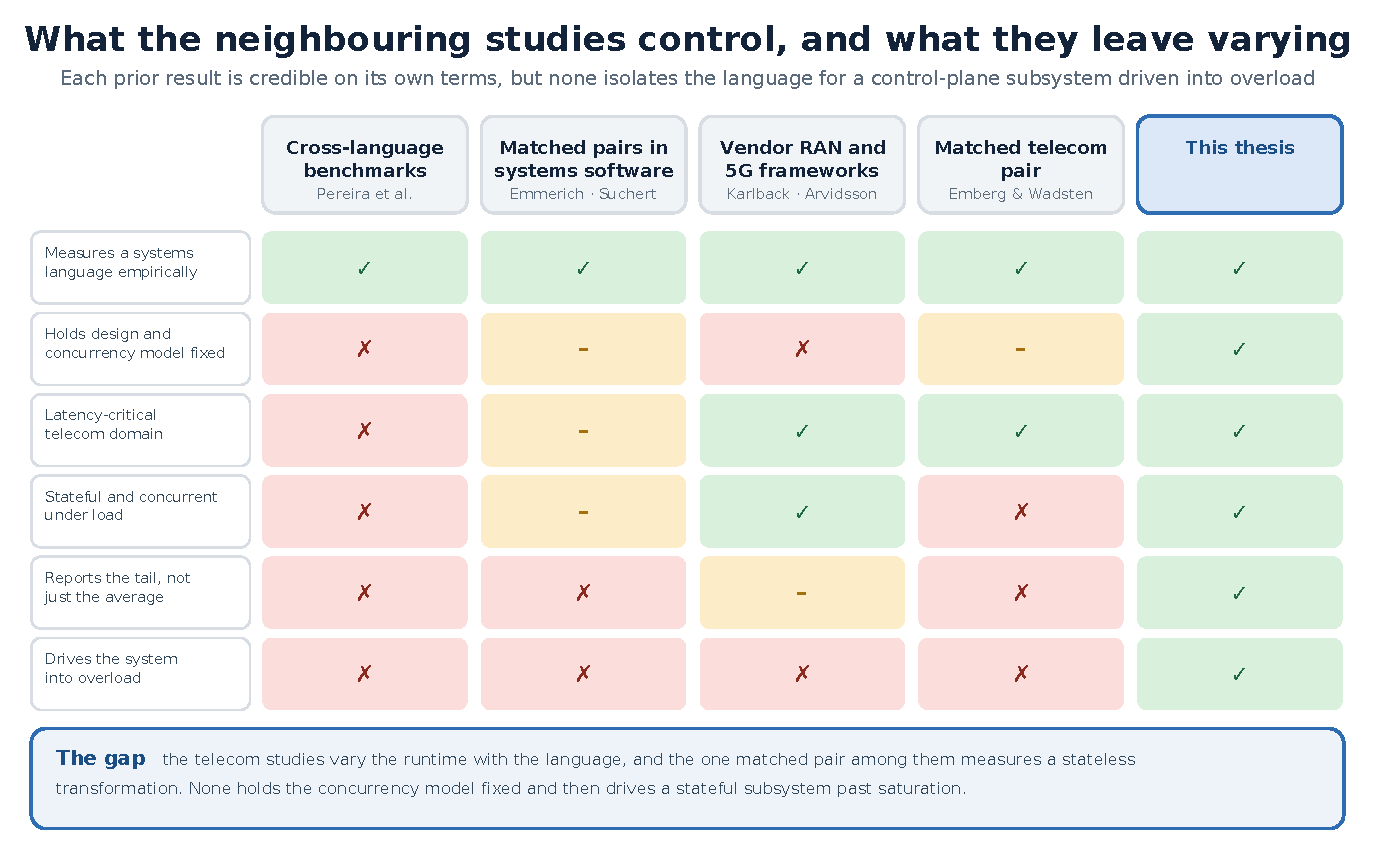
\includegraphics[width=0.78\linewidth]{diagrams/pdf/29_research_gap.pdf}
\caption[Các nghiên cứu lân cận kiểm soát gì, và để gì biến thiên]{Các nghiên cứu lân cận kiểm
soát gì, và để gì biến thiên. Mỗi hàng là một thuộc tính mà một câu trả lời có kiểm soát sẽ
cần, và mỗi cột là một nhóm nghiên cứu. Cột RAN nhà cung cấp là các luận văn Ericsson trừ
Emberg và Wadsten, những người có cột riêng vì họ giữ thiết kế sát hơn.\label{fig:gapmap}}
\end{figure}

Điều còn thiếu trong công trình trước là một phép thử trực tiếp, có kiểm soát, trên một phần
mặt điều khiển điển hình. Các câu hỏi mở như sau. Rust có giữ độ trễ đuôi khi tải quá lớn đối
với C++ hiện đại khi mô hình luồng, thao tác và bố cục dữ liệu được giữ cố định? Nó loại những
lớp lỗi nào, và phần còn lại bị bắt ở giai đoạn nào? Mô hình an toàn của nó tốn gì về thông
lượng và về CPU cùng bộ nhớ? Áp dụng từng bước tốn gì trên thực tế? Đóng khoảng trống này là
mục đích của bốn câu hỏi nghiên cứu. Chương tiếp theo neo chúng vào phần đang được nghiên cứu,
các lớp lỗi, và thời gian đang bị đe dọa. Nó cũng nêu phương pháp.

\chapter{Phương pháp nghiên cứu\label{chapter:methodology}}
\chaptermark{Phương pháp}

Chương trước nêu khoảng trống. Chương này nêu cách nghiên cứu đóng nó.

\section{Phân hệ Quản lý Ngữ cảnh UE}\label{sec:uecm}
Phần được nghiên cứu là một dịch vụ Quản lý Ngữ cảnh UE. Nó được mô hình hoá theo một dịch vụ
gNB-CU-CP thực của Nokia, sở hữu vòng đời ngữ cảnh UE, thực thi thủ tục
RRC~\cite{3gpp38331}, và di động cùng chuyển giao. Đó là các chức năng mà thiết kế 3GPP giao
cho phần mặt điều khiển của một gNB tách (Mục~\ref{sec:ranarch}). Hình~\ref{fig:fsm} cho thấy
vòng đời ngữ cảnh UE mà cả hai bản mã hoá cùng một cách. Khối lượng hỗn hợp của
Mục~\ref{sec:workload} đưa mỗi UE đi qua máy trạng thái đó.

\begin{figure}[ht]
\centering
\begin{tikzpicture}[
    ->, >=Stealth, node distance=3.2cm, font=\small,
    every state/.style={draw, minimum size=1.5cm, fill=blue!6, thick},
    every edge/.style={draw, thick}
  ]
  \node[state, initial, initial text=\scriptsize tạo] (idle) {Idle};
  \node[state, right=of idle] (conn) {Connected};
  \node[state, right=of conn] (reconf) {Reconf.};
  \node[state, below=1.9cm of conn, fill=gray!10] (rel) {Released};

  \path (idle)  edge node[above,font=\scriptsize]{setup} (conn)
        (conn)  edge[bend left=18] node[above,font=\scriptsize]{begin} (reconf)
        (reconf) edge[bend left=18] node[below,font=\scriptsize]{complete / abort} (conn)
        (conn)  edge node[right,font=\scriptsize,pos=0.45]{release} (rel)
        (idle)  edge[bend right=32] node[below,font=\scriptsize,pos=0.6]{release} (rel);
  \path (conn) edge[loop above] node[font=\scriptsize]{signal / add DRB} (conn);
\end{tikzpicture}
\caption[Máy trạng thái vòng đời ngữ cảnh UE]{Máy trạng thái vòng đời ngữ cảnh UE.
Các thao tác không hợp lệ với trạng thái hiện tại trả về lỗi thay vì đổi
trạng thái.\label{fig:fsm}}
\end{figure}

UECM là công việc tầng 3 RAN cốt lõi. Nó có những đặc tính làm mã mặt điều khiển đang chạy trở
nên khó. Mỗi UE có trạng thái thay đổi. Vòng đời thao tác chặt. Nhiều UE chạy cùng lúc. Mục
tiêu trễ là những mục tiêu hệ thống 5G đặt cho thủ tục mặt điều
khiển~\cite{3gpp38913,3gpp22261}. Phát hiện về cách một ngôn ngữ xử lý những đặc tính đó liên
quan nhất tới các dịch vụ mặt điều khiển nhiều luồng, có trạng thái khác cùng loại. Phần này
cũng đủ nhỏ để đặc tả trọn vẹn và xây hai lần. Đó là điều làm một phép so sánh có kiểm thử
tương đương trở nên khả thi.

Giao diện nhỏ và được xây quanh vòng đời. Nó có thể tạo và giải phóng một ngữ cảnh. Nó có thể
thiết lập một kết nối. Nó có thể xử lý một thông điệp báo hiệu trong phiên. Nó có thể thêm một
data radio bearer. Nó có thể bắt đầu, hoàn tất, hoặc huỷ một tái cấu hình. Nó có thể tra trạng
thái của một ngữ cảnh dưới tải. Mỗi thao tác được định nghĩa cho mỗi trạng thái của
Hình~\ref{fig:fsm}. Một thao tác bất hợp pháp trả về lỗi có kiểu và để ngữ cảnh không đổi. Tập
đóng đó cho phép cùng các kiểm thử và cùng khối lượng đưa cả hai bản đi theo cùng các đường.

RQ2 cần một danh mục, không phải một danh sách mối nguy lỏng. Một danh mục được xây từ tập thao
tác này: $\FaultClasses$ lớp trong hai nhóm bảy. Bảy lớp đến từ bên trong vùng mà Rust an toàn
tuyên bố cai quản. Bảy lớp được chọn vì Rust an toàn được kỳ vọng không ngăn chúng. Mỗi lớp có
kỳ vọng được ghi trước khi các chương trình chạy. Mục~\ref{sec:safetyresults} báo cáo mỗi lớp
đã làm gì.

Đuôi là chỉ số vì hai đặc tính của phần này. Một hành động người dùng nhìn thấy, thiết lập cuộc
gọi hoặc chuyển giao, thành nhiều thao tác mặt điều khiển phụ thuộc nhau. Thành viên chậm nhất
chặn hoàn tất. Một site bận đưa hàng nghìn thủ tục như vậy mỗi giây. Vì vậy một điểm đuôi xa
được chạm đủ thường để có ý nghĩa. Dạng thất bại là lý do thứ hai. Một dịch vụ thiết kế này
theo tải đưa vào với độ trễ phẳng cho đến khi một luồng xử lý bão hoà. Rồi độ trễ nhảy mạnh
trong một bước tải. Đó là lý do nghiên cứu này quét qua bão hoà.

\section{Hướng tiếp cận nghiên cứu}\label{sec:approach}
Nghiên cứu chạy thí nghiệm. Nó cũng xây thứ nó đo: một cặp bản khớp nhau, cộng khung đo đưa
chúng chạy. Cả hai được xây từ một đặc tả cố định. Bằng chứng đến từ ba phương pháp tách biệt.
Một quét tải trả lời RQ1 và RQ3. Tiêm lỗi có kiểm soát trả lời RQ2. Một nguyên mẫu di trú FFI
trả lời RQ4. Một điểm yếu ở một trong số chúng, chẳng hạn máy chủ có thể dịch chuyển đuôi bao
nhiêu, không lan sang phần còn lại của các tuyên bố.

Mỗi câu hỏi hỏi một kết quả phụ thuộc vào một biến, ngôn ngữ. Ngôn ngữ phải là khoảng cách có
kế hoạch duy nhất giữa hai đối tượng thử. Điều đó loại trừ cách so sánh ngôn ngữ phổ biến nhất.
Ở dạng đó hai chương trình viết độc lập được đo, và khoảng cách được lấy là ngôn ngữ. Khoảng
cách đó cũng mang thiết kế, thư viện, và kỹ năng của tác giả. Xây cả hai phía từ một đặc tả loại
nhiễu loạn đó. Ở nơi câu hỏi trả lời được bằng số, nó dùng số. Ở nơi không thể, câu trả lời vẫn
theo một kế hoạch cố định, bằng lời. Đó là cách nghiên cứu này xử lý loại bảo đảm trong RQ2.
RQ4 hỏi về chi phí thiết kế của giao diện lập trình ứng dụng (API).

Công trình trước gần nhất là năm luận văn do nhà cung cấp lưu trữ của
Mục~\ref{sec:gap}. Chúng không xuất hiện trong cơ sở dữ liệu trích dẫn nào. Chúng phải được tìm
bằng cách tra kho lưu trữ của từng trường bằng tay. Cùng các tìm kiếm đó không tìm thấy luận
văn Phần Lan nào về Rust trong bối cảnh truy nhập vô tuyến. Chúng không tìm thấy bài được lập
chỉ mục nào nhắc Rust từ nhà cung cấp chủ trì công trình này. Tìm kiếm không trả về nghiên cứu
nào đo đuôi của một bản Rust và một bản C++ của cùng một phần mặt điều khiển nhiều luồng, có
trạng thái, dưới tải quá lớn.

Bảng~\ref{tab:design} ánh xạ mỗi câu hỏi nghiên cứu tới phương pháp, hiện vật, dữ liệu và chỉ
số trả lời nó. RQ1 và RQ3 dùng chung H1, diễn đạt để phủ một hoà tốc độ theo cả nghĩa trễ và
nghĩa tài nguyên. Cách diễn đạt đó hoá ra là điểm yếu chính của giả thuyết. RQ2 không phụ thuộc
máy chủ. RQ4 phụ thuộc theo một trục. Thời gian biên dịch là một phép đo thời gian. Vì vậy nó
được đọc như tỉ số giữa hai chuỗi công cụ đo luân phiên trên một máy.

\begin{table}[ht]
\centering
\small
\caption[Cách mỗi câu hỏi nghiên cứu được trả lời]{Cách mỗi câu hỏi nghiên cứu được trả lời.
RQ1 và RQ3 mang hai phương pháp chứ không phải một: quét đo vòng khứ hồi mà một triển khai sẽ
trải, và tách lõi khỏi bàn giao đo phần mà ngôn ngữ chịu trách nhiệm.
\label{tab:design}}
\renewcommand{\arraystretch}{1.2}
\setlength{\tabcolsep}{4pt}
\begin{tabular}{@{}p{0.07\linewidth} p{0.27\linewidth} p{0.27\linewidth} p{0.27\linewidth}@{}}
\hline\hline
RQ & Phương pháp & Hiện vật / dữ liệu & Chỉ số chính \\
\hline
RQ1 & Quét tải tới quá tải, lặp đan xen & Khung đo, histogram độ trễ &
trung vị, p99/p99.9/p99.99, và cực đại so với tải đưa vào \\
RQ3 & Cùng quét, thu tài nguyên & Mẫu \texttt{getrusage} mỗi lần chạy &
kích thước tập trú (RSS) đỉnh, CPU, thông lượng \\
RQ1, RQ3 & Gọi lõi trực tiếp, rồi qua dịch vụ &
Cặp microbenchmark khớp &
thao tác đối với bàn giao giữa luồng \\
RQ2 & Tiêm lỗi có kiểm soát & Danh mục lỗi, ba bộ dò lỗi C++,
\texttt{rustc}, Loom/Shuttle, Miri &
biên dịch / lúc chạy / không phát hiện \\
RQ4 & Nguyên mẫu di trú FFI & Máy chủ C++ $+$ đường nối C-ABI Rust &
kích thước đường nối, phạm vi \texttt{unsafe}, chi phí mỗi lần gọi \\
\hline
\end{tabular}
\end{table}

\section[Phương pháp theo từng câu hỏi]{Phương pháp theo từng câu hỏi nghiên cứu, tóm tắt}\label{sec:methodbrief}
RQ1 và RQ3 được trả lời bằng một quét tải vòng hở từ tải nhẹ đến vượt xa bão hoà. Vòng hở nghĩa
là bộ sinh giữ lịch gửi của nó thay vì chờ trả
lời~\cite{schroeder2006openclosed}. Bốn biến thể build được đan xen trong mỗi lần lặp. Một phép
đo thời gian thứ hai tách thao tác lõi khỏi bàn giao giữa luồng quanh nó. Vòng khứ hồi đầu-cuối
gói hai chi phí thuộc hai loại. Chỉ một trong hai có thể khác giữa các ngôn ngữ. Một phép đo
thứ ba lấy hàng đợi tranh chấp và tay cầm trả lời riêng. Vì vậy nguyên nhân quá tải có thể được
thử chứ không chỉ được lập luận.

RQ2 được trả lời bằng tiêm lỗi có kiểm soát~\cite{natella2016fault}. Mỗi lớp lỗi là một chương
trình nhỏ riêng ở cả hai ngôn ngữ. Phía C++ được xây và chạy dưới AddressSanitizer. Nó cũng
chạy dưới ThreadSanitizer và UndefinedBehaviorSanitizer. Phía Rust an toàn được biên dịch và,
nơi nó biên dịch, chạy dưới một hạn thời gian bị chặn. Không bộ phân tích tĩnh nào được chạy,
cố ý. Các cột C++ khi đó báo cáo công cụ mà nghiên cứu này đã chạy. Chúng không báo cáo trần
của những gì công cụ C++ có thể tìm. RQ4 được trả lời bằng một nguyên mẫu chạy được theo hướng
một cuộc di trú thực đi. Một máy chủ C++ gọi một lõi Rust không đổi qua ABI C. Chi phí mỗi lần
gọi được đo trên một thao tác thực chứ không suy từ một lần vượt trống. Lỗi bộ nhớ vượt ngôn
ngữ nằm ở đường nối đó~\cite{li2022crosslang}.

\section{Tính công bằng như một biến được kiểm soát}\label{sec:controlsbrief}
Một phép so sánh ngôn ngữ chỉ tốt bằng các biến nó giữ cố định. Đặc tả được cố định trước khi
bản nào tồn tại. Mô hình luồng, bộ cấp phát và số arena của nó, mức tối ưu, hàm băm, phương
pháp histogram và lịch tải được khớp giữa hai phía. Chúng không bao giờ được tinh chỉnh theo
từng phía. Nơi hai ngôn ngữ không thể viết giống nhau, khoảng cách được ghi lại chứ không được
hoà. Hai phía được chứng minh khớp bằng cách diff nhật ký khớp theo từng thao tác. Một hàng của
bảng đó không có đối chứng. Một người viết cả hai bản và không thành thạo như nhau ở cả hai.
Mục~\ref{sec:standing} coi đó là mối đe dọa nội tại chính của nghiên cứu.

\section{Xử lý thống kê}\label{sec:statsbrief}
Thiết kế thống kê được cố định trước. Họ các phép so sánh được thử được liệt kê trước chiến
dịch. Vì vậy một mức tải chọn sau khi nhìn một quét không thể vào họ. Mỗi phép so sánh là một
kiểm định hoán vị ghép cặp chính xác trên \NRepeats{} lần lặp đan xen, với khoảng tin cậy
bootstrap~\cite{efron1993bootstrap}, hiệu chỉnh Holm trên cả
họ~\cite{holm1979simple}. Các sàn mà kiểm định có thể đạt ($\MinAttainableP$ chưa hiệu chỉnh,
$\CorrectedFloor$ đã hiệu chỉnh) được nêu để một kết quả null phân biệt được với một giới hạn
toán. Hai đại lượng được giữ ngoài họ. Một là độ dao động từ lần gọi này sang lần gọi khác, mà
không câu hỏi nghiên cứu nào hỏi. Đại lượng kia là đuôi xa p99.99 gộp. Đơn vị của nó là thao
tác, không phải lần chạy. Nó khi đó không có khoảng giữa các lần lặp để thử.

\section{Tái lập và hiện vật nghiên cứu}\label{sec:repro}
Một bên thứ ba có thể xây lại kết quả mà không cần mã riêng của Nokia. Các bản được đưa chạy
hoàn toàn bởi đặc tả công khai đã cố định. Khung đo, danh mục lỗi và bộ chạy của nó, và nguyên
mẫu FFI được công bố cùng luận văn. Mỗi hình dữ liệu đo được một kịch bản xây lại từ nhật ký
thô. Mỗi số được trích trong kết quả cũng vậy. Kịch bản đó là
\texttt{bench/refresh\_thesis.sh}. Tuyên bố đó không phủ các sơ đồ vẽ tay, vốn giải thích một
khái niệm chứ không báo cáo một kết quả. Và chạy cùng các kịch bản trên chiến dịch của một máy
khác xây lại hiện vật theo cùng thủ tục, không với cùng giá trị.

Các nhật ký mà kịch bản đọc là một phần của gói. Mỗi chiến dịch có kịch bản riêng và tiền tố
macro riêng, nên một hình từ chiến dịch này không thể chạm một câu về chiến dịch kia. Thiết lập
máy chủ của mỗi lần chạy được ghi và lưu cạnh dữ liệu chiến dịch. Không gì trong các chương kết
quả được gõ từ những tệp đó bằng tay.

\chapter{Thiết kế và hiện thực\label{chapter:design}}
\chaptermark{Thiết kế}

Không gì được xây cho đến khi đặc tả được cố định. Nó chốt giao diện lập trình công khai, máy
trạng thái UE, bố cục dữ liệu và các bước trên đó, khoá và kích thước phân mảnh, và mô hình
luồng. Cả hai bản đều bám theo nó. Phép thử khi đó đo ngôn ngữ, không phải một khoảng cách thiết
kế hay kỹ năng. Bản thân đặc tả là một đầu ra của nghiên cứu. Nó là kiểm soát chính chống thiên
lệch của người viết.

Một mô hình luồng được dùng ở cả hai phía: không chia sẻ trạng thái và một luồng mỗi phân mảnh.
Bố cục đó được biết là tự nó đổi độ trễ đuôi~\cite{enberg2019threadpercore}. Không gian định
danh được tách thành các phân mảnh. Mỗi phân mảnh thuộc một luồng xử lý. Chỉ luồng đó đọc hoặc
đổi nó. Vì vậy không khoá nào canh trạng thái ngữ cảnh. Bên gọi gửi một yêu cầu tới hàng đợi bị
chặn của phân mảnh sở hữu. Chúng chờ trên một tay cầm trả lời một lần. Hàng đợi chặn khi đầy.
Điều đó là cố ý. Một quy tắc bỏ sẽ che quá tải. Nghiên cứu này cần quá tải hiện ra như độ trễ.
Trạng thái khả biến dùng chung duy nhất mà bản nào cho phép là một bộ đếm nguyên tử. Không luồng
điều khiển nào phụ thuộc giá trị của nó. Hình~\ref{fig:arch} cho thấy luồng dữ liệu. Có một hàng
đợi nhiều tác nhân sinh, một tác nhân tiêu thụ (MPSC) mỗi phân mảnh. Luồng xử lý của nó rút theo
vào trước ra trước (FIFO).

\begin{figure}[ht]
\centering
\begin{tikzpicture}[
    font=\small,
    prod/.style={draw, rounded corners, minimum width=2.0cm, minimum height=0.66cm, fill=blue!8},
    queue/.style={draw, minimum width=2.5cm, minimum height=0.66cm, fill=gray!12},
    worker/.style={draw, rounded corners, minimum width=2.1cm, minimum height=0.66cm, fill=red!8},
    store/.style={draw, cylinder, shape border rotate=90, aspect=0.25, minimum width=1.5cm, minimum height=0.85cm, fill=green!8},
    lane/.style={draw, dotted, rounded corners, inner sep=7pt},
    >={Stealth[length=2.4mm]}
  ]
  \node[prod] (p1) at (0,1.3)  {Tác nhân 1};
  \node[prod] (p2) at (0,0.0)  {Tác nhân 2};
  \node[prod] (p3) at (0,-1.3) {Tác nhân $m$};
  \begin{scope}[on background layer]
    \node[draw, dashed, rounded corners, fill=blue!3, fit=(p1)(p2)(p3), inner sep=6pt] (pg) {};
  \end{scope}
  \node[font=\scriptsize] at (0,-2.15) {bộ sinh tải};

  \node[queue] (q1) at (5.2,1.3)   {Hàng đợi MPSC};
  \node[worker](w1) at (8.9,1.3)   {Worker 1};
  \node[store] (s1) at (12.0,1.3)  {Phân mảnh 1};
  \node[queue] (qn) at (5.2,-1.3)  {Hàng đợi MPSC};
  \node[worker](wn) at (8.9,-1.3)  {Worker $n$};
  \node[store] (sn) at (12.0,-1.3) {Phân mảnh $n$};
  \begin{scope}[on background layer]
    \node[lane, fit=(q1)(s1)] (lane1) {};
    \node[lane, fit=(qn)(sn)] (lanen) {};
  \end{scope}
  \node[font=\scriptsize] at (8.35,2.35) {luồng sở hữu phân mảnh: không trạng thái khả biến dùng chung, không khoá};

  \node[font=\scriptsize, align=center, fill=white, inner sep=2pt] at (2.85,0) {định tuyến theo\\ hash(\texttt{ue\_id})};
  \draw[->] (pg.east) -- (q1.west) node[midway, above, sloped, font=\scriptsize]{gửi};
  \draw[->] (pg.east) -- (qn.west) node[midway, below, sloped, font=\scriptsize]{gửi};

  \draw[->]  (q1) -- node[above, font=\scriptsize]{FIFO} (w1);
  \draw[->]  (qn) -- node[above, font=\scriptsize]{FIFO} (wn);
  \draw[<->] (w1) -- node[above, font=\scriptsize]{sở hữu} (s1);
  \draw[<->] (wn) -- node[above, font=\scriptsize]{sở hữu} (sn);

  \draw[->, dashed, rounded corners=4pt]
      (wn.south) -- ++(0,-0.75) -- (1.4,-2.9) -- ($(pg.south east)+(-0.4,0)$);
  \node[font=\scriptsize] at (5.9,-3.05) {hoàn tất một lần (kết quả $\rightarrow$ tác nhân đang chờ)};
\end{tikzpicture}
\caption[Kiến trúc không chia sẻ, một luồng mỗi phân mảnh]{Kiến trúc không chia sẻ, một luồng
mỗi phân mảnh. Các tác nhân sinh gửi vào một hàng đợi MPSC bị chặn mỗi phân mảnh, và luồng xử
lý của phân mảnh đó rút hàng.\label{fig:arch}}
\end{figure}

Tính công bằng được giữ dưới thiết kế cũng như trong thiết kế. Cả hai bản build liên kết cùng
\texttt{jemalloc}. Cả hai giữ một bản build bộ cấp phát hệ thống làm đối chứng. Cả hai biên dịch
ở cùng mức tối ưu. Cả hai ghi độ trễ qua một bộ histogram dải động cao (HDR) được lập cùng một
cách~\cite{tene_hdrhistogram}. Băm được chốt ở cả hai phía. SplitMix64 gán phân mảnh. FNV-1a,
hàm băm Fowler--Noll--Vo, được dùng bên trong bảng. Hàm băm mặc định của C++ trên một số nguyên
thường chỉ là chính số đó. Của Rust mạnh là cố ý. Để nguyên như chúng đến, hai thư viện chuẩn
sẽ là phép đo.

Nơi các ngôn ngữ không thể đáp một nhu cầu cùng một cách, khoảng cách được viết vào nhật ký
thành ngữ bắt buộc rồi được đo. Hai trong số các khoảng cách đó mang kết quả quá tải của
Mục~\ref{sec:overload}. Một là hàng đợi bị chặn. Rust lấy nó từ \texttt{sync\_channel}. C++23
vẫn chưa có nguyên thủy đó, nên C++ xây một cái từ một mutex và hai biến điều kiện. Cái kia là
tay cầm trả lời, \texttt{std::promise} đối với một kênh \texttt{mpsc} mới mỗi yêu cầu. Một
khoảng cách thứ ba mang kết quả thao tác lõi của Mục~\ref{sec:perfresults}: container mỗi phân
mảnh là bảng băm chuẩn của chính ngôn ngữ đó. Một khoảng cách thứ tư là mã hoá yêu cầu. C++
không có kiểu liệt kê mang payload theo thành ngữ này, nên một yêu cầu thành một struct có nhãn
giữ mỗi trường mà thao tác nào cũng có thể cần, $\CppRequestBytes$~byte đối với
$\RustRequestBytes$ của Rust. Kết quả ròng là một lõi Rust dài hơn $\NlocRise\%$ về dòng mã. Độ
phức tạp cyclomatic của nó thấp hơn $\CcnTotalDrop\%$~\cite{lizard}. Thư viện Rust không chứa
\texttt{unsafe} nào cả.

Tương đương được thử chứ không được giả định. Các vector trung lập ngôn ngữ chạy ở cả hai bản.
Nhật ký của chúng được diff theo từng thao tác. Một diff chéo không phân biệt ``cả hai đúng''
với ``cả hai sai cùng một cách''. Một bản thứ ba bằng Python đóng vai tiên tri độc lập. Nó phải
tái tạo tất cả $\ConfHandOps$ kỳ vọng suy bằng tay trước khi được sinh kỳ vọng của riêng mình.
Một chiến dịch $\ConfGenOps$ thao tác được sinh không tìm thấy lệch. Phía C++ chạy dưới
AddressSanitizer, ThreadSanitizer và UndefinedBehaviorSanitizer. Phía Rust chạy dưới Miri. Một
kết quả bộ dò lỗi sạch bị chặn bởi mã thực sự đã chạy.

\chapter{Thiết lập thí nghiệm và đánh giá\label{chapter:eval}}
\chaptermark{Đánh giá}

Chương này bắt đầu với các máy thử và khối lượng công việc. Kết quả rồi theo chế độ tải, rồi
theo các câu hỏi nghiên cứu còn lại.

\section{Thiết lập hệ thống thử\label{sec:testbed}}
Một số số trong chương này đến từ trình biên dịch và mã. Các số khác phụ thuộc máy chúng chạy
trên. Mọi số tốc độ ở đây đến từ một máy chủ vật lý chuyên dụng, một socket \MainCpu{}. Mỗi nhân
chạy một luồng. Đa luồng đồng thời là \MainSmt{}. Máy chạy \MainHostDistro{} trên nhân
\MainKernel{}. Linux có thể tăng và giảm xung mỗi nhân khi tải và nhiệt đổi. Xung được giữ cố
định: bộ điều tần là \MainGovernor{}, và boost tắt. Benchmark chỉ được dùng các nhân
\MainPinned{}. Không có hypervisor, nên chương trình chạy trên chính máy chứ không trong một máy
ảo. Trên các nhân đó nhân hệ điều hành tắt ngắt thời gian định kỳ (\texttt{nohz\_full}). Những
ngắt đó nếu không sẽ hiện trong các số độ trễ. Nghiên cứu không dùng \texttt{isolcpus}. Cờ đó
cũng ngăn nhân rải việc trên các nhân được phép. Mọi luồng benchmark khi đó đáp xuống một nhân.

Các trình biên dịch không phải những cái cài trên máy chủ. Cả hai bản được xây và chạy trong một
ảnh container mang \MainDistro{} với \texttt{g++~\MainGpp} và \texttt{rustc~\MainRustc}. Ảnh chốt
phiên bản chính \texttt{gcc-toolset} chứ không phải bản phát hành trong đó. Chiến dịch trước trên
một máy ảo vì vậy biên dịch với \texttt{g++~\GuestGpp}, sớm hơn một bản phát hành GNU Compiler
Collection (GCC)~15. Một container vẫn dùng nhân của máy nó ngồi trên. Hai chiến dịch khi đó
khác nhau về phần cứng, về nhân (\MainKernel{} đối với \GuestKernel{}), và về bản phát hành trình
biên dịch đó.

Cho đến muộn trong công việc, chiến dịch chạy trên một máy ảo thay vì vậy: Kernel-based Virtual
Machine (KVM) trên một \GuestCpu{}, không có các kiểm soát nhân ở trên. Trên máy đó khoảng tin
cậy $95\%$ trên p99 của một biến thể đơn trải $\GuestPNineNineMaxCI\,\mu$s, trong khi giá trị
p99 của bốn biến thể lệch $\GuestPNineNineRange\,\mu$s. Nhiễu trên một biến thể lớn hơn khoảng
cách giữa cả bốn. Chiến dịch đó được giữ. Nó dùng cùng thiết kế với chiến dịch này, nên hai bên
có thể được so để hỏi phát hiện nào thuộc về mã. Một quét thứ ba trên một máy vật lý thứ hai
\BmCpu{} dùng số phân mảnh, lưới tải, số lần lặp và trình biên dịch khác. Nó thử liệu các phát
hiện có sống sót những thay đổi đó cùng nhau, không phải từng cái tách riêng.

\section[Khối lượng và phép đo]{Khối lượng công việc và phép đo\label{sec:workload}}
Khối lượng được làm cho thí nghiệm. Các bước nó đi lấy từ quy tắc
3GPP~\cite{3gpp38401,3gpp38331}. Một bộ lái luôn gửi cùng chuỗi đưa mỗi UE qua vòng đời kết nối
mà các quy tắc đó định. Khối lượng \emph{signal} trước hết kết nối một tập UE, rồi gửi cùng thao
tác báo hiệu hết lần này đến lần khác. Điều đó cô lập đường phổ biến. Khối lượng \emph{mixed} đưa
mỗi UE qua tạo ngữ cảnh, thiết lập, báo hiệu, thiết lập bearer, tái cấu hình hoặc chuyển giao,
và giải phóng. Một thứ tự ngẫu nhiên cố định làm cả hai ngôn ngữ thấy cùng số đếm mỗi loại thao
tác cho một hạt giống cho trước. Đó cũng là một kiểm tra rằng hai bản đã làm cùng việc.
Hình~\ref{fig:workload} cho thấy hai khối lượng và chuỗi mà khối mixed đi.

\begin{figure}[ht]
\centering
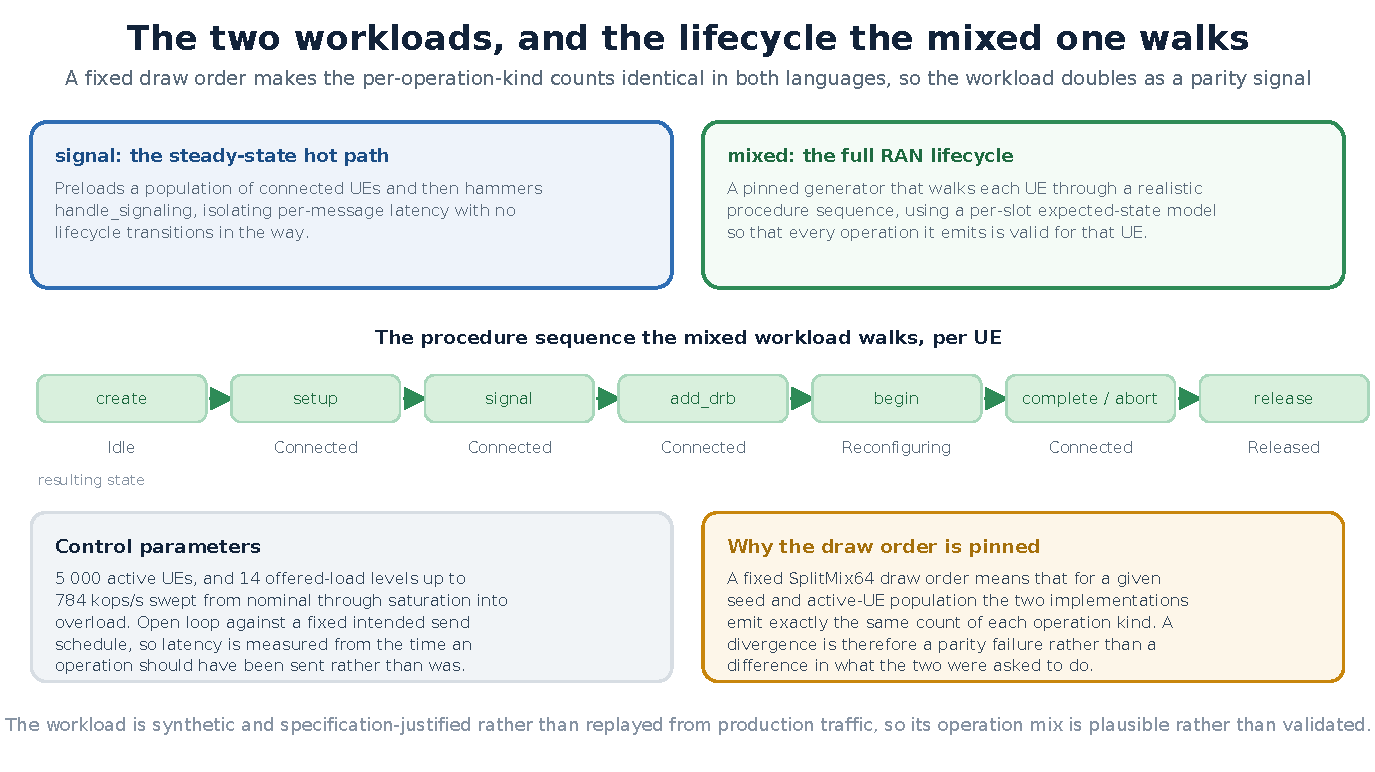
\includegraphics[width=0.78\linewidth]{diagrams/pdf/27_workload_timeline.pdf}
\caption[Hai khối lượng, và vòng đời mà khối mixed đi]{Hai khối lượng, và vòng đời mà khối mixed
đi. Signal lặp đường phổ biến, và mixed đưa mỗi UE qua chuỗi thủ tục vẽ
dưới.\label{fig:workload}}
\end{figure}

Chuỗi thao tác khớp quy tắc 3GPP. Tần suất mỗi loại xuất hiện thì không. Một cell thực chuyển
giao thường đến mức nào phụ thuộc site và giờ trong ngày, và không con số công khai nào chốt nó.
Một hỗn hợp không khớp một cell thực dịch cả hai ngôn ngữ cùng một lượng. Nó giới hạn mức các số
đi xa được. Nó không làm phép so sánh bất công. Bộ gửi giữ lịch của nó dù dịch vụ trễ (vòng hở),
và histogram được hiệu chỉnh, nên một tắc không che các trả lời thiếu (thiên lệch bỏ sót phối
hợp)~\cite{schroeder2006openclosed}. Mỗi mức tải được lặp \NRepeats{} lần. Bốn biến thể ngôn ngữ
và bộ cấp phát được đan xen trong mỗi lần lặp. Mỗi điểm báo cáo là một trung vị với khoảng tin
cậy bootstrap $95\%$~\cite{georges2007rigorous,efron1993bootstrap}.

Tải dùng cho các hình tài nguyên là $\ReprLoad$~kilo-thao-tác mỗi giây (kops/s). Đó là một giá
trị được chọn, không phải một giá trị tính từ quét. Quy tắc đầu tiên nghiên cứu này dùng là mức
tải bận nhất mà p99 ở dưới $5$~ms. Trên máy ảo quy tắc đó đáp xuống nhiễu của máy chủ. Trên một
máy yên nó leo cho đến khi dịch vụ không còn theo kịp. Nó được giữ chỉ như một kiểm tra. Cao
nguyên thông lượng thấp nhất trong bốn biến thể là $\SatKnee$~kops/s, đạt khi tải đưa vào là
$\TrackingLoad$~kops/s.

\section{Kết quả}
Các kết quả an toàn và phần lớn kết quả di trú không phụ thuộc máy nào được dùng. Các kết quả
tốc độ và bộ nhớ thì có. Mỗi hình dưới đây được đo trên máy chủ của Mục~\ref{sec:testbed} trừ
khi chú thích nói khác.

\subsection{Dưới bão hoà (RQ1, RQ3)}\label{sec:perfresults}
Khi dịch vụ vẫn theo kịp tải đưa vào, trung vị của bốn biến thể nằm trong $\PFiftyRange\,\mu$s
của nhau, $\PFiftySpread\%$. Một kiểm định ghép cặp vẫn tìm thấy khác biệt
$\PFiftyDiffAbsMax\,\mu$s nghiêng về Rust dưới cả hai bộ cấp phát. Hình~\ref{fig:loadsweep} cho
thấy quét đứng sau điều đó. Các phân vị cao hơn nay cũng đọc được. Khoảng rộng nhất trên p99 của
một biến thể đơn trải $\PNineNineMaxCI\,\mu$s. Giá trị p99 của bốn biến thể lệch
$\PNineNineRange\,\mu$s. Vì vậy nhiễu trên một cái nhỏ hơn khoảng cách giữa chúng. Trên máy ảo
cùng hai đại lượng đó là $\GuestPNineNineMaxCI\,\mu$s đối với $\GuestPNineNineRange\,\mu$s, theo
chiều ngược. Cả hai hàng p99 và cả hai hàng p99.9 vượt hiệu chỉnh Holm, \NTailSignificant{} hàng
tất cả, cùng chiều với trung vị. Bảng~\ref{tab:latency} báo cáo p99.9 và cực đại tại tải đại
diện. Cực đại được giữ ngoài họ được thử, như p99.99 gộp.

\begin{table}[ht]
\centering
\small
\caption[Độ trễ mỗi thao tác tại tải đại diện]{Độ trễ mỗi thao tác, tính bằng micro giây, tại
$\ReprLoad$~kops/s. Trung vị trên \NRepeats{} lần lặp nằm trên khoảng bootstrap $95\%$ của nó.
$^{\dagger}$Cột p99.99 được gộp giữa các lần lặp, nên không có khoảng. Cực đại được giữ ngoài họ
được thử vì cùng lý do.\label{tab:latency}}
\LatencyTabular
\hline\hline
\LatencyHead \\
\hline
C++ (system alloc) & \mci{217.2}{163.8}{237.2} & \mci{355.1}{289.3}{389.4} & \mci{674.3}{395.3}{1538.0} & \mci{2170}{910}{5594} \\
C++ (jemalloc) & \mci{225.8}{181.1}{261.2} & \mci{410.1}{305.7}{11280.4} & \mci{1188}{544}{14213} & \mci{3590}{1472}{16291} \\
Rust (system alloc) & \mci{214.3}{191.6}{238.8} & \mci{376.3}{330.2}{3629.1} & \mci{1068}{504}{6955} & \mci{2404}{1129}{9667} \\
Rust (jemalloc) & \mci{208.4}{193.7}{223.1} & \mci{388.9}{342.3}{478.0} & \mci{763.4}{479.5}{4272.1} & \mci{2804}{1114}{7606}
\\
\hline
\end{tabular}
\end{table}

\begin{figure}[ht]
\centering
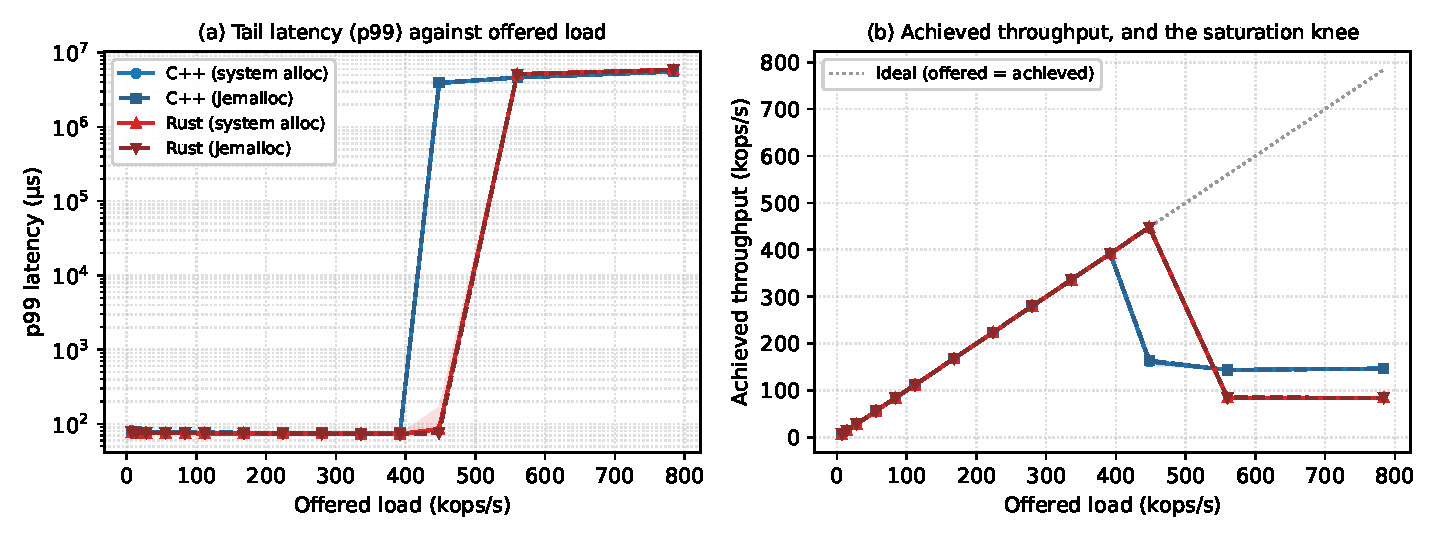
\includegraphics[width=0.78\linewidth]{figures/fig_load_sweep.pdf}
\caption[Quét tải: độ trễ đuôi và thông lượng đạt được]{Quét tải, cả hai tấm đối với tải đưa
vào. Đường là trung vị trên \NRepeats{} lần lặp, và dải là khoảng tin cậy bootstrap
$95\%$.\label{fig:loadsweep}}
\end{figure}

Đuôi xa cũng đọc được ở đây. Histogram của các lần lặp được gộp, cho \FarTailSamplesMin{} đến
\FarTailSamplesMax{} thao tác mỗi biến thể. Hai biến thể \FarTailLower{} nằm dưới cả hai biến
thể C++. Cặp rộng nhất lệch $\FarTailRange\,\mu$s. Biến thể Rust chậm nhất vẫn nằm
$\FarTailLangSep\,\mu$s dưới biến thể C++ nhanh nhất. Một máy vật lý thứ hai ở số phân mảnh khác
đồng ý, chạy $\BmFarTailCppLo$--$\BmFarTailCppHi\,\mu$s cho các biến thể C++ đối với
$\BmFarTailRustLo$--$\BmFarTailRustHi\,\mu$s cho các biến thể Rust, không chồng. Một giới hạn thứ
hai không đến từ máy. Không máy chủ nào xoá được giới hạn đó. Một vòng khứ hồi đầu-cuối chỉ dành
$\BudgetCoreShareMax\%$ thời gian cho công việc ngôn ngữ thực hiện. Phần còn lại là đưa yêu cầu
sang luồng khác, và thời gian đó được tính cho hệ điều hành. Khi công việc bên trong ngôn ngữ
nhỏ như vậy, thời gian vượt biên luồng chiếm ưu
thế~\cite{zhou2025oltp}. Quét này không thể giới hạn một hiệu ứng ngôn ngữ theo chiều nào, điều
mà Hình~\ref{fig:budget} đặt cạnh những gì quét vẫn còn cho thấy. Đo riêng, thao tác lõi nhanh
hơn $\BudgetCoreRatio\times$ ở \BudgetCoreFaster{}. Nguyên nhân khả dĩ là cách bảng băm
chuẩn được bố trí, không phải mô hình an toàn.

\begin{figure}[ht]
\centering
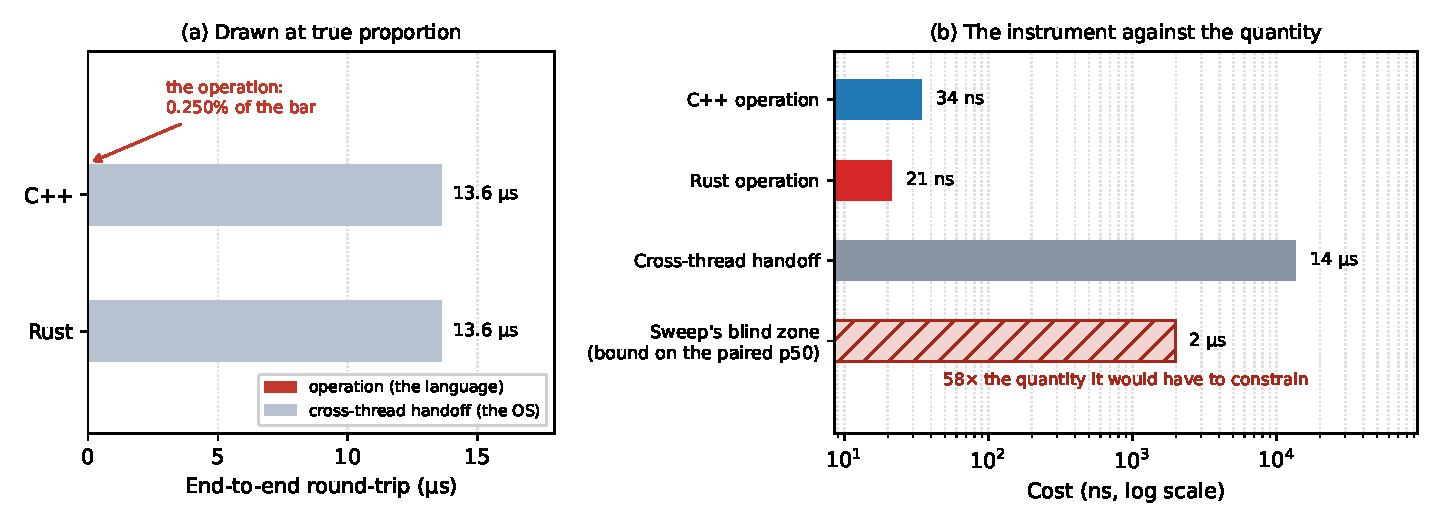
\includegraphics[width=0.78\linewidth]{figures/fig_budget.pdf}
\caption[Thao tác đầu-cuối được phân rã, đối với những gì quét phân giải được]{Chi phí của một
vòng khứ hồi đầu-cuối đi đâu. \textbf{(a)} Vòng khứ hồi ở tỉ lệ thật. \textbf{(b)} Cả hai phép
đo thao tác nằm trong vùng mù của quét theo hệ số $\BudgetBoundVsCore$.\label{fig:budget}}
\end{figure}

\subsection{Qua bão hoà (RQ1)}\label{sec:overload}
Khi tốc độ đưa vào cao hơn dịch vụ chịu được, bốn biến thể ngừng theo kịp ở các tải khác nhau.
Các bản Rust giữ đến $\TrackingLoadRust$~kops/s. Các bản C++ giữ đến $\TrackingLoadCpp$. Vì vậy
tại $\KneeGapLoad$~kops/s \KneeGapFaster{} vẫn phục vụ $\KneeGapThrFast$~kops/s nơi
\KneeGapSlower{} đã rơi xuống $\KneeGapThrSlow$. Mức tải đó được mô tả chứ không được thử, vì nó
được tìm sau khi dữ liệu đã có.

Sâu hơn, tại $\OverloadLoad$~kops/s đưa vào, thứ tự đảo. \OverloadSustainedFaster{} vẫn hoàn
thành $\OverloadThrCpp$~kops/s nơi \OverloadSustainedSlower{} hoàn thành $\OverloadThrRust$, một
hệ số $\OverloadThrRatio$, trong \OverloadThrAgree{} lần lặp dưới cả hai bộ cấp phát. Giá trị
$p$ đã hiệu chỉnh Holm nhỏ đến mức họ kiểm định này có thể đi. Biến thể chậm hơn không chỉ làm
ít việc hơn. Nó dùng $\OverloadCpuPerOpRatio$ lần CPU cho mỗi thao tác nó hoàn thành, dấu hiệu
của nỗ lực bỏ ra mà không hoàn tất gì. Khi hàng đợi bị chặn và tay cầm hoàn tất được đo riêng,
thứ tự đó không có ý nghĩa, nên nguyên nhân nằm trên đường rộng hơn đưa việc giữa các luồng.
Đây là hiệu ứng ngôn ngữ lớn nhất trong họ được thử. Một phép so sánh dừng ở tải mà dịch vụ vẫn
đáp sẽ chỉ theo chiều kia. Hình~\ref{fig:overload} đặt những gì mỗi biến thể vẫn hoàn thành cạnh
những gì nó tốn để hoàn thành.

\begin{figure}[ht]
\centering
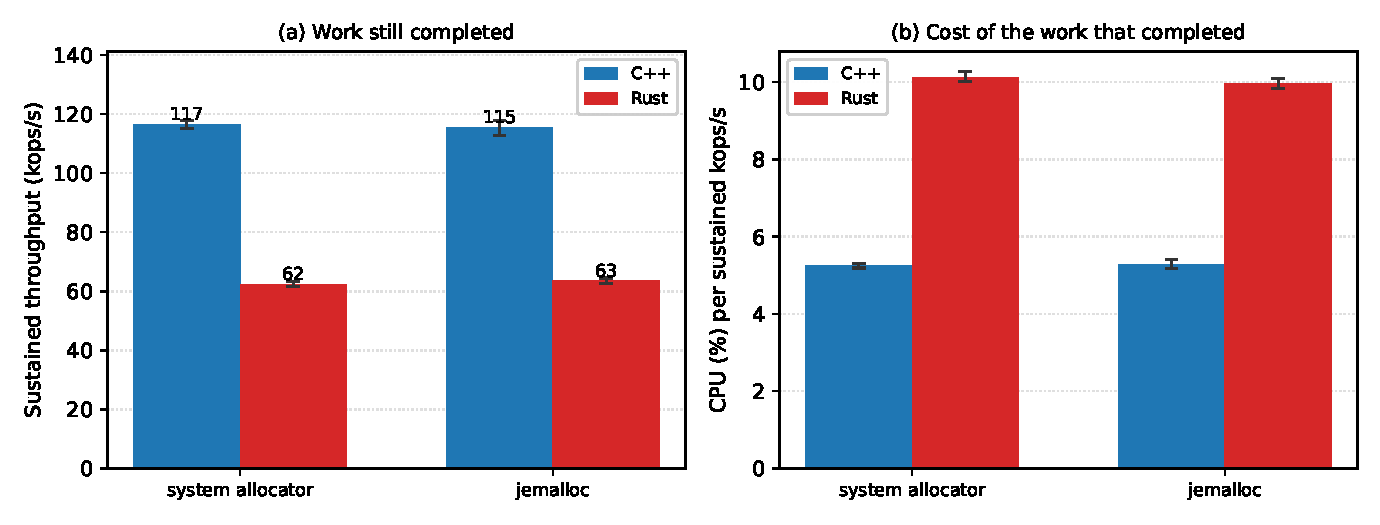
\includegraphics[width=0.78\linewidth]{figures/fig_overload.pdf}
\caption[Phân kỳ qua bão hoà]{Hành vi tại $\OverloadLoad$~kops/s đưa vào. Cột là trung vị trên
\NRepeats{} lần lặp với khoảng bootstrap $95\%$, nhóm sao cho hai cột trong một nhóm chỉ khác
ngôn ngữ. CPU trong (b) được cộng trên các luồng.\label{fig:overload}}
\end{figure}

\subsection{Dùng tài nguyên (RQ3)}\label{sec:resources}
Bộ nhớ và CPU tách các biến thể nơi độ trễ không tách được. Hai hiệu ứng cỡ tương đương nằm
trong RSS đỉnh. Bản build Rust dùng $\RssLangDiffLo$--$\RssLangDiffHi$~MiB bộ nhớ đỉnh nhiều hơn
bản build C++ dưới bộ cấp phát nào. Liên kết \texttt{jemalloc} nói chung tốn
$\RssAllocDiffLo$--$\RssAllocDiffHi$~MiB ở ngôn ngữ nào. Cả hai đều thực, và
Hình~\ref{fig:resources} đặt cặp đó cạnh RSS đỉnh mà chúng cộng thành. Hiệu ứng ngôn ngữ giữ
chiều và cỡ trên cả ba máy được đo. Của bộ cấp phát là $\GuestRssAllocOverLang$ lần hiệu ứng ngôn
ngữ trên máy ảo nghiên cứu này dùng trước ($\GuestRssAllocLo$--$\GuestRssAllocHi$~MiB), nên tỉ
số của chúng phụ thuộc máy. Khác biệt ngôn ngữ là chi phí cố định, không phải chi phí mỗi UE.
Máy yên là nơi điều đó nhìn thấy được. Bộ đếm của chính \texttt{jemalloc} ở đó đặt
$\BmJeMetadataDelta$~MiB nhiều hơn vào sổ sách arena và $\BmJeAllocatedDelta$~MiB \emph{ít hơn}
vào cấp phát còn sống. Byte trú của nó thấp hơn $\BmJeResidentDelta$~MiB. Đỉnh tiến trình cao
hơn $\BmJeRssDelta$~MiB. Bộ nhớ thêm khi đó nằm ngoài bộ cấp phát, trong thời gian chạy mà một
tiến trình Rust mang trước khi nó cấp phát. CPU đổi dấu theo tải. Tại tải đại diện
$\ReprLoad$~kops/s Rust dùng ít hơn tối đa $\CpuDiffAbsMax$ điểm phần trăm. Khi dịch vụ không
còn theo kịp, CPU mỗi thao tác hoàn thành cao hơn nhiều.

\begin{figure}[ht]
\centering
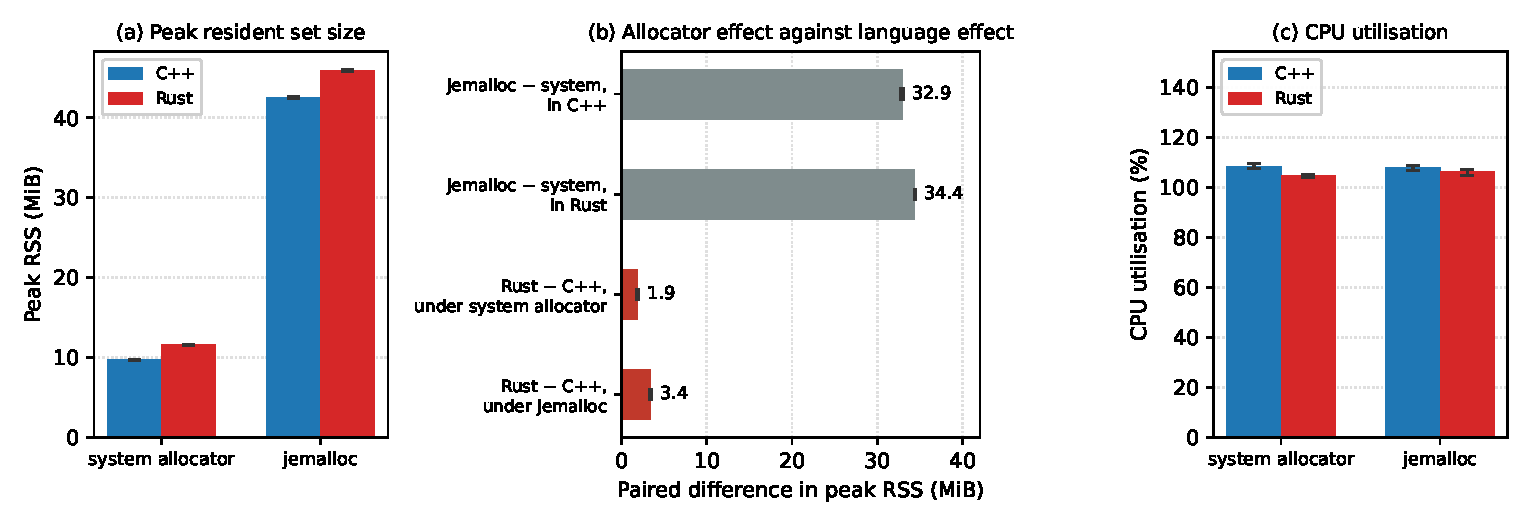
\includegraphics[width=0.78\linewidth]{figures/fig_resources.pdf}
\caption[Dùng tài nguyên, và hai hiệu ứng trong RSS đỉnh]{Dùng tài nguyên tại
$\ReprLoad$~kops/s, nhóm theo bộ cấp phát. Cột là trung vị trên \NRepeats{} lần lặp với khoảng
bootstrap $95\%$, và CPU trong (c) được cộng trên các luồng.\label{fig:resources}}
\end{figure}

\subsection{An toàn qua tiêm lỗi (RQ2)}\label{sec:safetyresults}
An toàn được đo bằng cách tiêm $\FaultClasses$ lỗi. Bảy lớp đến từ bên trong vùng Rust tuyên bố
cai quản. Bảy lớp được chọn vì Rust an toàn được kỳ vọng \emph{không} ngăn chúng. Mỗi lớp trong
bảy lớp đầu là lỗi biên dịch ở Rust. Ở C++ mỗi lớp là mã hợp lệ. Lỗi chỉ hiện nếu một kiểm thử
đưa nó chạy, và không bộ dò lỗi đơn nào phủ chúng. Use-after-move là trường hợp không bộ dò lỗi
nào báo gì. Một đối tượng đã move vẫn là một đối tượng hợp lệ. Giá trị của nó không xác định.
Vì vậy không có gì bất hợp pháp để phát hiện, và định danh đơn giản là mất. Cả bảy trường hợp
biên đều biên dịch trong Rust an toàn và hành xử sai. Trên hai lớp trong số đó công cụ C++ là
bên báo. LeakSanitizer gắn cờ chu trình tham chiếu mà Rust rò trong im lặng, vì rò là an toàn
trong Rust theo thiết kế tường minh~\cite{hughes2025gcrust,cui2024rcanary}.
UndefinedBehaviorSanitizer gắn cờ overflow mà Rust định nghĩa là quấn. ThreadSanitizer bắt đảo
thứ tự khoá trong $\DeadlockTsanHits$ trên $\DeadlockTsanRuns$ lần chạy, một tỉ lệ bản thân không
ổn định. Nó chỉ ghi thứ tự khoá từ các khoá thành công. Nếu lần đảo đầu chờ mãi, chu trình không
bao giờ đóng, nên công cụ không bao giờ báo.

Double-free đường nối là double-free trong bảo đảm viết lại qua \texttt{unsafe}, không phải một
lớp mới. Nửa C++ của nó không đổi, nên chỉ cột Rust dịch. Hai bộ kiểm tra mô hình Rust có báo cả
hai lỗi biên gốc. Loom duyệt xen kẽ luồng một cách vững. Shuttle lấy mẫu những xen kẽ Loom không
với tới~\cite{bornholt2021shardstore}. Mỗi cái phải được viết bằng nguyên thủy của chính bộ kiểm
tra trước, và thu nhỏ về cỡ mô hình. Miri báo double-free đường nối, nhưng nó diễn giải Rust và
không chạy được máy chủ C++ mà lỗi nằm sau. LeakSanitizer và UndefinedBehaviorSanitizer báo mà
không cần viết lại. Hai bộ kiểm tra mô hình chỉ báo các trường hợp biên tương tranh sau khi lỗi
được viết lại vào nguyên thủy của chúng. Hình~\ref{fig:taxonomy} vẽ cả danh mục như một ma trận
kết cục. Resource Acquisition Is Initialization (RAII) gỡ việc quên mở khoá thông thường. Nó không
gỡ lớp: cả hai chương trình quên guard đều treo, và công cụ của ngôn ngữ nào cũng không nói vậy.

\begin{figure}[ht]
\centering
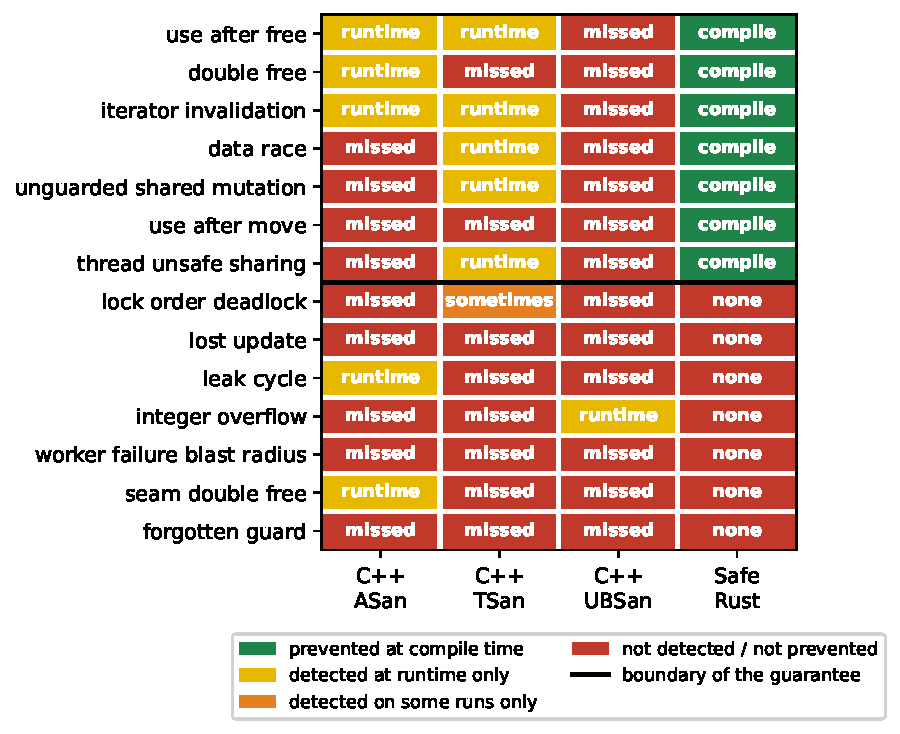
\includegraphics[width=0.72\linewidth]{figures/fig_taxonomy.pdf}
\caption[Nơi bảo đảm dừng: ma trận kết cục]{Kết cục tiêm lỗi như một ma trận, sinh từ nhật ký
phân loại.\label{fig:taxonomy}}
\end{figure}

\subsection{Di trú (RQ4)}\label{sec:migrationresults}
Đường nối di trú nhỏ trên mỗi trục được đo: $\FfiEntryPoints$ điểm vào C trong $\FfiSeamLines$
dòng Rust. Mọi việc con trỏ thô bị nhốt trong $\FfiUnsafeFns$ hàm. Lõi được để không
\texttt{unsafe}. Không chi phí thêm nào được phát hiện đối với cùng cuộc gọi báo hiệu thực hiện
trực tiếp. Điều đó giới hạn mọi thuế mỗi lần gọi ở $\FfiOpBoundPct\%$ của cuộc gọi đó, và
Hình~\ref{fig:ffiseam} cho thấy cấu trúc mà giới hạn đó thuộc về. Ba chi phí áp dụng ngoài đường
nối cũng được đo, và hai trong số đó mâu thuẫn với phản đối thường gặp khi áp dụng Rust.
$\BuildDepShareCpu\%$ của lần build sạch Rust là mã bên thứ ba. Mã nguồn của chính dự án biên
dịch trong $\BuildAllFirstPartyCpuRatio$ lần CPU mà \texttt{g++} cần. Khoảng cách kích thước nhị
phân $\FootShippedRatio\times$ là một chính sách liên kết đảo chiều khi chính sách được giữ cố
định. Thành phần được so sánh không có crate bên thứ ba và không có vị trí \texttt{unsafe}
($\DepsCore$ crate, $\CoreUnsafe$ vị trí \texttt{unsafe}).

\begin{figure}[ht]
\centering
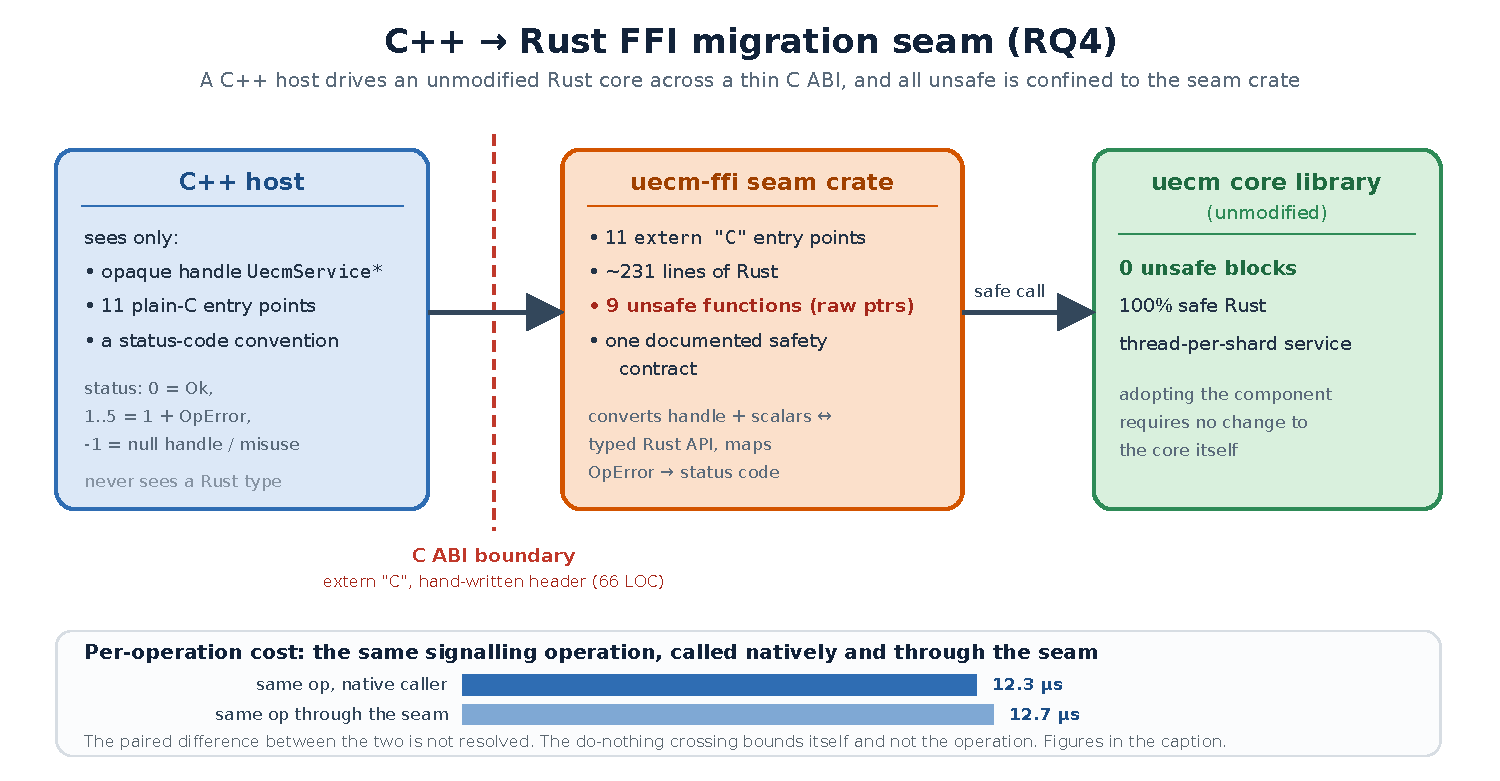
\includegraphics[width=0.78\linewidth]{diagrams/pdf/07_ffi_seam.pdf}
\caption[Đường nối di trú FFI từ C++ sang Rust]{Đường nối di trú FFI từ C++ sang Rust. Cùng thao
tác báo hiệu tốn $\FfiOpNative$~\textmu s trực tiếp và $\FfiOpSeam$~\textmu s qua đường nối, một
khác biệt ghép cặp được giới hạn ở $\FfiOpBoundPct\%$ của cuộc gọi đó. Một lần vượt không làm gì
tốn $\FfiCrossing$~ns và chỉ giới hạn chính nó.\label{fig:ffiseam}}
\end{figure}

\chapter{Thảo luận\label{chapter:discussion}}

\section{Tóm tắt phát hiện}
Câu trả lời cho RQ1 chia tại bão hoà. Dưới đó các biến thể khớp nhau đến $\PFiftyRange\,\mu$s ở
trung vị, và đuôi xa phân giải nghiêng về \FarTailLower{}. Vòng khứ hồi đầu-cuối chỉ là
$\BudgetCoreShareMax\%$ công việc ngôn ngữ, nên nó không thể giới hạn một hiệu ứng ngôn ngữ.
Cùng thao tác đo riêng nhanh hơn $\BudgetCoreRatio\times$ ở \BudgetCoreFaster{}. Qua bão hoà
chúng phân kỳ theo cả hai chiều. Các nhánh Rust giữ tốc độ đưa vào đến $\TrackingLoadRust$~kops/s
đối với $\TrackingLoadCpp$. Tại $\OverloadLoad$~kops/s \OverloadSustainedFaster{} duy trì
$\OverloadThrRatio\times$ thông lượng của \OverloadSustainedSlower{}.
RQ2 là kết quả đã chốt và không phụ thuộc máy chủ. Cả bảy lớp trong bảo đảm đều là lỗi biên dịch
trong Rust an toàn. Cả bảy lớp biên đều biên dịch và hành xử sai ở cả hai ngôn ngữ. RQ3 là một
phạt bộ nhớ $\RssLangDiffLo$--$\RssLangDiffHi$~MiB tái hiện dưới cả hai bộ cấp phát và trên cả
ba máy, với CPU đảo dấu qua hai chế độ tải. RQ4 là một đường nối nhỏ mà thuế mỗi lần gọi được
giới hạn ở $\FfiOpBoundPct\%$ của cuộc gọi đó. Chi phí thực là thiết kế API và đường cong học
tập.

\section{Thảo luận các câu hỏi nghiên cứu}\label{sec:rqdiscussion}
Việc một triển khai nên làm gì với RQ1 phụ thuộc nơi nó kỳ vọng ngồi, không phụ thuộc một xếp
hạng đơn. Một dịch vụ được định cỡ để chạy dưới điểm gối của mỗi nhánh nên chọn nhánh giữ tốc độ
đưa vào xa hơn. Một dịch vụ mà một cơn bão báo hiệu sẽ đẩy qua mỗi điểm gối nên chọn nhánh vẫn hoàn
thành nhiều việc hơn sau đó. Hai ưa thích đó hướng tới hai ngôn ngữ đối lập. Chỉ cái thứ hai
được thử. Cái thứ nhất là mô tả, vì lý do Mục~\ref{sec:overload} đưa. Một phép so sánh dừng ở
tải mà dịch vụ vẫn đáp sẽ đọc chiều ngược với cùng bộ máy.

Công trình trước gần nhất đo đại lượng này cho các thủ tục mặt điều khiển 5G. Nó tìm cùng hình
dạng và truy nó về \texttt{async}/\texttt{await} không ngăn xếp~\cite{arvidsson2025async}. Quy
kết đó được chấp nhận ở đây. Hình dạng xuất hiện mà không có thời gian chạy bất đồng bộ ở phía
nào và mô hình tương tranh được giữ cố định. Một thời gian chạy không thể là nơi duy nhất một
hiệu ứng như vậy phát sinh. Dự đoán đăng ký trước cũng nêu nơi nhìn trước, kiểm biên và kiểm
overflow~\cite{zhang2022runtime,harris2023morello}. Phần đó của nó sai. Khoảng cách trung vị
khớp với bằng chứng rằng các kiểm an toàn của Rust phần lớn được CPU hiện đại ra-khỏi-thứ-tự
hấp thụ~\cite{balasubramanian2017rust,emmerich2019drivers}. Nó cũng yếu hơn vẻ ngoài. Thao tác
lõi là $\BudgetCoreShareMax\%$ những gì quét đo.

Về an toàn, một số lỗi không thể chạm một nhị phân chút nào. Bảy lớp Rust không ngăn là một phần
của câu trả lời, không phải một cảnh báo thêm sau. Một trình biên dịch từ chối xây một chương
trình loại lỗi khỏi mỗi lần thực thi. Một bộ dò lỗi chỉ loại nó khỏi những lần chạy mà một kiểm
thử bộ dò lỗi tình cờ đi. Cái tuyệt đối ở đó là phủ thực thi, không phải bề rộng của danh mục.
Hình~\ref{fig:boundary} nêu cơ chế mỗi bên của đường đó. Rust lý luận về aliasing chứ không về
thứ tự chiếm. Một guard \texttt{Mutex} mà bộ kiểm mượn theo dõi vòng đời hoàn hảo không nói gì
về việc hai luồng lấy khoá theo thứ tự tương thích. Phát hiện khoá chết tĩnh cho Rust là một bài
toán nghiên cứu đang mở~\cite{zhang2026deadlock}. Lost update thoát ThreadSanitizer vì cùng lý
do nó thoát bộ kiểm mượn. Nơi mỗi truy cập được đồng bộ đúng, không có truy cập không đồng bộ để
tìm. Trong một nghiên cứu hiện trường $105$ lỗi tương tranh thực, khoảng một phần ba các trường
hợp không phải khoá chết vi phạm thứ tự lập trình viên định chứ không phải việc
khoá~\cite{lu2008mistakes}. Áp dụng Rust loại một hạng lỗi tương tranh và để nguyên hạng thất
bại trong im lặng. Một kế hoạch di trú đọc ``an toàn bộ nhớ'' như ``an toàn tương tranh'' sẽ
tính sai ngân sách rà soát. Lỗi an toàn bộ nhớ trong Rust dính \texttt{unsafe} trong mọi mục
Common Vulnerabilities and Exposures (CVE) đã công bố trừ một lỗi trình biên
dịch~\cite{xu2021rustcve}, đó là lý do giữ lõi không \texttt{unsafe} quan trọng, và lý do
mã \texttt{unsafe} lan qua phụ thuộc là mối quan tâm rà soát~\cite{evans2020rust}.

\begin{figure}[ht]
\centering
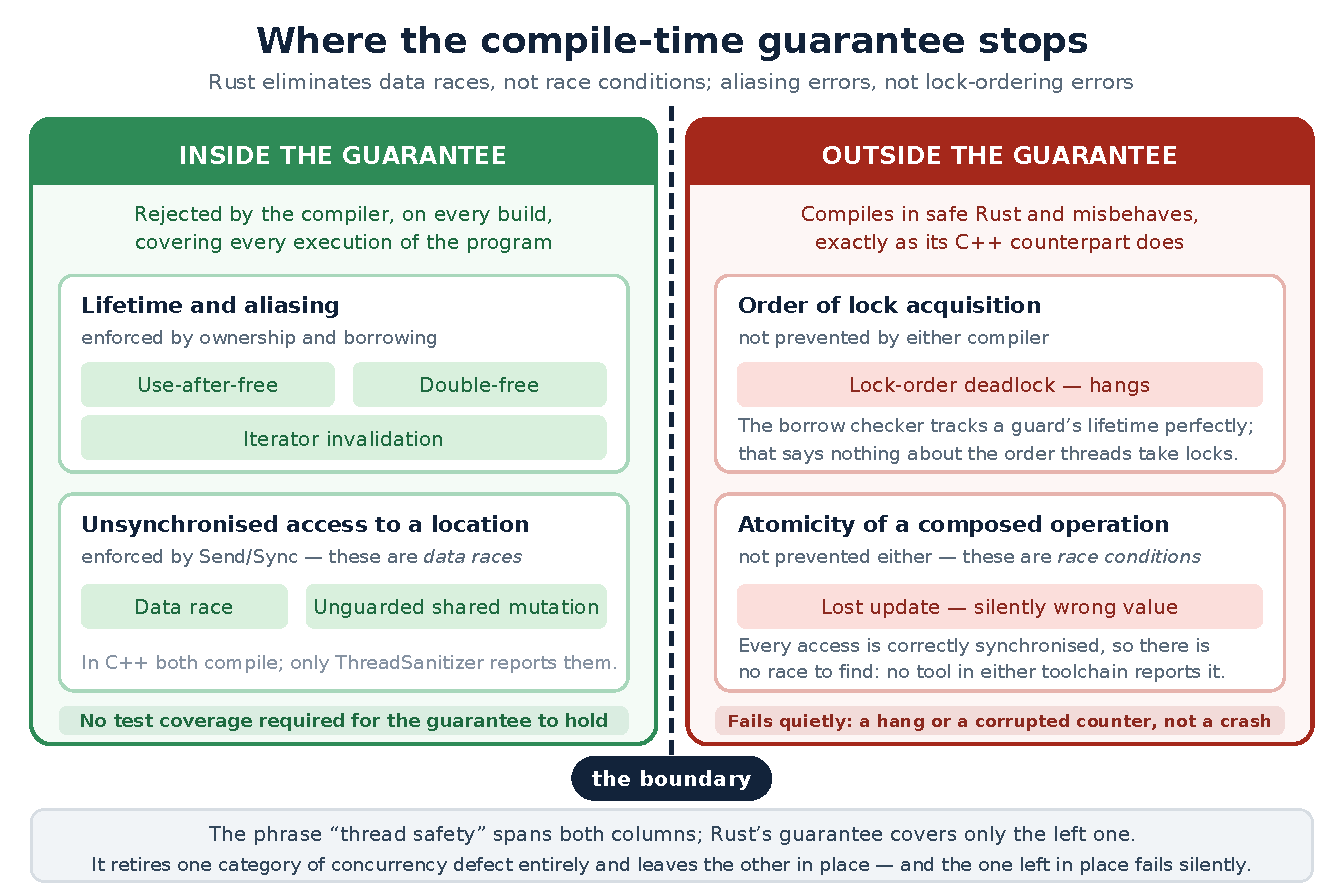
\includegraphics[width=0.78\linewidth]{diagrams/pdf/17_guarantee_boundary.pdf}
\caption[Nơi bảo đảm lúc biên dịch của Rust dừng]{Nơi bảo đảm lúc biên dịch của Rust dừng, các
lớp nhóm theo cơ chế từ chối chúng.\label{fig:boundary}}
\end{figure}

Một trường hợp vượt quá các chương trình được tiêm. Một lỗ đặc tả cho phép một thao tác được gửi
ngoài cửa sổ chạy của dịch vụ. Nó sống sót mỗi kiểm thử, mỗi vector tương đương và cả ba bộ dò
lỗi vì không gì từng gọi đường đó. Cái biến hành vi không định nghĩa thành một thất bại chẩn
đoán được ở phía Rust là một kiểm biên thông thường, không phải một chứng minh. Thuộc tính đáng
ngân sách là ``được kiểm mặc định'', không phải ``bị loại lúc biên dịch''. Nguyên nhân gốc thuộc
về phương pháp. Một cấm nêu ra mà không có cơ chế phía sau để mỗi bản thất bại theo thành ngữ
của riêng nó.

RQ3 tách theo tài nguyên và các tách không chỉ cùng chiều. Phạt bộ nhớ tái hiện dưới cả hai bộ
cấp phát và trên một máy thứ hai với trình biên dịch khác. Tập trú đỉnh là cực đại cấp lần chạy,
nên độ dao động phá một p99 không chạm nó. Đo so với hiệu ứng của chính bộ cấp phát, hai cái
cùng bậc trên cả hai máy vật lý. Trên máy ảo, của bộ cấp phát lớn hơn một bậc. Hiệu ứng ngôn
ngữ đi được. Tỉ số thì không. Máy yên cũng định vị chi phí ngoài bộ cấp phát, bằng sổ sách của
chính bộ cấp phát. Một nghiên cứu gần báo dấu ngược, Rust thấp nhất và khoảng cách rộng khi
tương tranh tăng~\cite{karlback2021ran}. Hai phát hiện đó khớp nhau khi các nhánh được đọc như
hai thời gian chạy tương tranh. C++ của họ chạy trên Boost.Fibers, cấp một ngăn mỗi fiber. Rust
của họ chạy trên Tokio, nơi một task là một future nhỏ cấp trên heap. Họ đo chi phí mỗi ngữ cảnh
của hai thời gian chạy tương tranh. Hai nghiên cứu nữa khớp chiều tìm thấy ở
đây~\cite{olsson2023ranmgmt,sundvisson2026drivers}. Về CPU dấu phụ thuộc tải. Một số đơn cho
``chi phí CPU của mô hình an toàn Rust'' sẽ trung bình hai chế độ đi ngược chiều.

RQ4 ra rẻ ở máy và đắt ở người. Một máy chủ C++ có thể gọi một lõi Rust không đổi qua một đường
nối C-ABI mỏng mà chi phí trên một cuộc gọi báo hiệu thực được giới hạn ở $\FfiOpBoundPct\%$ của
cuộc gọi đó. Chi phí chiếm ưu thế là con người~\cite{fulton2021adopting,crichton2024learning}. Nhốt
\texttt{unsafe} vào đường nối giới hạn những gì phải rà soát, không phải những gì có thể bị làm
hỏng. Máy chủ và thành phần chia một không gian địa
chỉ~\cite{rivera2021galeed,kirth2022pkrusafe}. Các trục build và dấu chân chỉ cùng chiều với
đường nối. Một nhà cung cấp lo một trong hai nên kiểm ngân sách phụ thuộc trước khi đổ lỗi trình
biên dịch. Trục duy nhất C++ dẫn thẳng là vòng sửa-biên dịch cho các thay đổi nằm trong một đơn
vị dịch. Con số kích thước nhị phân $\FootShippedRatio\times$ so hai chính sách liên kết, và thứ
tự đảo khi chính sách được giữ cố định.

\section{Xem lại các giả thuyết}\label{sec:hypotheses}
Mục~\ref{sec:rqs} cam kết ba giả thuyết trước mọi phép đo. Nêu cách xử chúng là điều tách một
phép thử khỏi một mô tả.

\begin{description}
  \item[H1] Mệnh đề trung vị giữ theo nghĩa thực tiễn. Kiểm định ghép cặp phân giải
        $\PFiftyDiffAbsMax\,\mu$s, quá nhỏ để giới hạn một hiệu ứng ngôn ngữ. Mệnh đề đuôi xa
        không giữ, và quá tải, điều mà cách diễn đạt không bao giờ nêu tên, là nơi các ngôn ngữ
        thực sự tách. Chiến dịch được báo cáo nay phân giải đuôi đó, nghiêng về Rust, và một máy
        vật lý thứ hai đồng ý về chiều. H1 đúng về nơi một khác biệt dưới bão hoà sẽ hiện và sai
        rằng đó là nơi duy nhất. Nó cũng không được đặt tốt. ``Tương đương hiệu năng'' đọc như
        một đại lượng và nêu ít nhất ba: vòng khứ hồi giao dưới bão hoà, mã các trình biên dịch
        phát, và việc bền dưới quá tải. Ba cái đó không đi cùng nhau.
  \item[H2] Với bảy lớp được tiêm cùng loại, nó giữ không ngoại lệ. Nó thất bại ở cách đọc lỏng
        hơn mà cách diễn đạt mời. Nó được chấp nhận cho an toàn bộ nhớ và không tranh chấp dữ
        liệu, bị bác cho tính đúng đắn tương tranh nói chung, và nó là tuyên bố chỉ về Rust
        \emph{an toàn}. Trường hợp đường nối cho thấy cùng lớp trở lại bên trong
        \texttt{unsafe}.
  \item[H3] Mọi thuế mỗi lần gọi được giới hạn ở $\FfiOpBoundPct\%$ của cuộc gọi báo hiệu đó, đó
        là chỗ dựa từ một giới hạn trên một chi phí mà phép đo có thể đã bỏ sót, không từ thất
        bại phát hiện một chi phí. Tuyên bố kèm theo, rằng chi phí thực là thiết kế và đào tạo,
        được chống đỡ về cấu trúc chứ không về thống kê.
\end{description}

\section{Hướng dẫn kỹ thuật cho áp dụng tăng dần}\label{sec:guidelines}
Các hướng dẫn là dạng thực tiễn của các phát hiện, và mỗi cái mang giới hạn của phát hiện đứng
sau. Chọn thành phần đầu vì giao diện hẹp, không vì kích thước. Thiết kế lại một giao diện giàu
là rủi ro lịch. Bản thân biên không phải. Giữ ABI C trong crate riêng và lõi không
\texttt{unsafe}. Điều đó giữ mã \texttt{unsafe} khỏi các chuỗi phụ thuộc mà nó nếu không lan
qua~\cite{evans2020rust}. Để ngân sách rà soát tương tranh ở chỗ cũ. Ưa một cấu trúc không chia
sẻ ở ngôn ngữ nào. Kết quả tương tranh mạnh nhất ở đây thuộc về thiết kế chứ không thuộc trình
biên dịch nào. Lập kế hoạch đường cong học tập như một chi phí đào tạo và đo nó. Đo thành phần
cũng như vòng khứ hồi. Quét qua điểm dịch vụ ngừng chịu được. Đó là hướng dẫn nghiên cứu này
muốn đã theo từ đầu nhất.

\section[Nơi nghiên cứu này đứng]{Nơi nghiên cứu này đứng, và những gì nó không chống đỡ được}\label{sec:standing}
Các nghiên cứu gần nhất với nghiên cứu này là năm luận văn do nhà cung cấp lưu trữ của
Mục~\ref{sec:gap}. Phán quyết của chúng mâu thuẫn nhau theo mỗi chiều. Bài báo dấu ngược trên
bộ nhớ đỉnh hoà với nghiên cứu này khi các nhánh được đọc như hai thời gian chạy tương tranh chứ
không phải hai ngôn ngữ. Ba mối đe dọa vẫn mang sức, và cái đầu là một tác giả viết cả hai bản.
Cùng dạng thất bại đã đảo một phán quyết đã công bố trong ngành này: tương đương sau một rà soát
mã rồi Rust kém hơn $85$--$91\%$ sau tối ưu thêm~\cite{emberg2023asn1}. Bộ tương đương chặn hành
vi chứ không chặn hiệu năng. Dụng cụ đầu-cuối đo thiết kế trung thành và ngôn ngữ hầu như không
đo. Phân kỳ quá tải được tái hiện ở đây với cơ chế được thu hẹp chứ không đóng, và không nghiên
cứu đã bình duyệt nào báo cùng sự đảo.

\section{Suy nghĩ đạo đức và nghề nghiệp}
Nghiên cứu không xử lý dữ liệu cá nhân, thuê bao, hay mật của nhà khai thác. Mọi lưu lượng đều
tổng hợp và phân hệ được mô hình hoá theo mã đang chạy chứ không sao chép từ đó, nên các hiện
vật có thể được phát hành công khai. Trách nhiệm thứ nhất là không tuyên bố quá. Một nhà cung
cấp có thể đọc kết quả RQ2 như giấy phép mô tả một thành phần đã di trú là ``an toàn'', và các
trường hợp biên là lý do cách đọc đó sai. Một mặt điều khiển khoá chết là một sự cố. Một cập
nhật bộ đếm mất trong im lặng có thể làm sai một quyết định di động. Không gì được chứng minh ở
đây ngăn một trong hai. Trách nhiệm thứ hai là bằng chứng đi xa đến đâu. Các số độ trễ đuôi từ
một máy đơn là cơ sở hẹp hơn vẻ ngoài cho một cam kết sản xuất. Đó là lý do chiến dịch máy ảo
trước được báo cáo chứ không bị loại.

\chapter{Kết luận và hướng phát triển\label{chapter:conclusions}}

Luận văn so sánh C++ hiện đại và Rust. Đối tượng là một dịch vụ Quản lý Ngữ cảnh UE mô hình hoá
theo một thành phần gNB-CU-CP thực của Nokia. Nó nhìn bốn chiều: khả năng dự đoán độ trễ đuôi,
ngăn lỗi lúc biên dịch, chi phí mô hình an toàn, và chi phí thêm Rust từng phần. Cả hai bản được
xây trên một đặc tả cố định và được đưa đi theo cùng các đường mã. Đó là điều cho phép tách một
hiệu ứng ngôn ngữ khỏi một khác biệt thiết kế hay kỹ năng.

Về an toàn, khác biệt là khác biệt về loại và nó có một biên rõ. Rust an toàn từ chối cả bảy
lớp an toàn bộ nhớ và tranh chấp dữ liệu được tiêm vào tại thời điểm biên dịch. Các mối nguy mà
C++ chỉ có thể hy vọng bắt dưới một kiểm thử bộ dò lỗi trở thành những chương trình không thể
viết. Cả bảy lớp biên đều biên dịch và hành xử sai trong Rust an toàn như trong C++. Trên hai
lớp trong số đó công cụ C++ báo những gì công cụ Rust không báo. Nêu chính xác, Rust loại tranh
chấp dữ liệu và lỗi aliasing. Nó không loại điều kiện đua, lỗi thứ tự khoá, rò rỉ, số học quấn
hay phạm vi thiệt hại của một luồng xử lý thất bại, và nó không loại gì bên trong một khối
\texttt{unsafe}. Nơi các lỗi biên bị bắt, chúng bị bắt lúc kiểm thử. LeakSanitizer và
UndefinedBehaviorSanitizer báo mà không cần viết lại. Hai bộ kiểm tra mô hình chỉ báo các trường
hợp tương tranh sau khi lỗi được viết lại vào nguyên thủy của chúng.

Về di trú, chi phí bị chiếm bởi thiết kế API và đường cong học tập, không bởi bất kỳ thuế lúc
chạy nào. Một lõi Rust không đổi có thể được điều khiển từ C++ qua một đường nối mỏng. Chi phí
trên một cuộc gọi báo hiệu thực được giới hạn ở $\FfiOpBoundPct\%$ của cuộc gọi đó. Toàn bộ
\texttt{unsafe} nằm ở đường nối, và lõi được xác nhận không có nó. Phần lớn chi phí thêm của lần
build Rust là biên dịch phụ thuộc, không phải công việc của chính trình biên dịch. Khoảng cách
kích thước nhị phân là một chính sách liên kết. Thứ tự phụ thuộc chính sách khớp nào được chọn.
Nơi C++ dẫn là vòng sửa-biên dịch, và nó chỉ dẫn với các sửa nằm trong một đơn vị dịch.

Về hiệu năng, bằng chứng chia trước theo cái đang được đo. Một vòng khứ hồi đầu-cuối ở đây là
$\BudgetCoreShareMax\%$ công việc ngôn ngữ. Phần còn lại là bàn giao của hệ điều hành. Đồng hồ
đó vì vậy không giới hạn gì về trình biên dịch nào. Cùng lõi đo riêng nhanh hơn
$\BudgetCoreRatio\times$ ở \BudgetCoreFaster{}. Tại tải đại diện $\ReprLoad$~kops/s, kiểm
định ghép cặp phân giải $\PFiftyDiffAbsMax\,\mu$s nghiêng về Rust, quá nhỏ để một triển khai bận
tâm ở trung vị. Tại p99.99 biến thể Rust chậm nhất nằm $\FarTailLangSep\,\mu$s dưới biến thể C++
nhanh nhất. Các nhánh Rust rồi giữ tốc độ đưa vào đến $\TrackingLoadRust$~kops/s đối với
$\TrackingLoadCpp$. Khi cả bốn đã sụp, \OverloadSustainedFaster{} duy trì
$\OverloadThrRatio\times$ thông lượng của \OverloadSustainedSlower{}, cái tốn
$\OverloadCpuPerOpRatio\times$ CPU trên mỗi thao tác nó hoàn thành. Về bộ nhớ, bản build Rust
mang thêm vài MiB dấu chân cố định dưới cả hai bộ cấp phát, cùng chiều và cùng cỡ trên cả ba máy
được đo. Lựa chọn bộ cấp phát tốn khoảng chừng đó trên cả hai máy vật lý, và nhiều hơn một bậc
trên máy ảo nghiên cứu này dùng trước.

Gộp lại, chúng ủng hộ một tuyên bố hẹp. Nó dành cho các dịch vụ mặt điều khiển có trạng thái,
tương tranh, phân vùng được thuộc loại này. Ở các tải mà dịch vụ vẫn đáp tốc độ đưa vào, lựa
chọn là những lớp lỗi nào một nhóm muốn làm không thể viết. Nửa kia là liệu nhóm sẽ trả chi phí
thiết kế và đào tạo để có chúng. Qua điểm đó nó cũng là một quyết định tốc độ. Điều luận văn
thêm là một dụng cụ đo, không phải một phán quyết. Dụng cụ đó là đặc tả cố định và cặp được kiểm
thử tương đương. Nó cũng là một khung đo thời gian đi qua điểm gối bão hoà. Một phép tách vòng khứ hồi nói
ngôn ngữ có thể chịu bao nhiêu phần của những gì khung đo. Một danh mục lỗi vẽ nơi bảo đảm dừng.

Công việc tương lai trả lời các khoảng trống từng cái một. Việc đầu không cần máy mới: đổi
chính sách transparent hugepage trên một máy chủ với mọi thứ khác giữ cố định. Cả ba máy đồng ý
rằng bản build Rust mang dấu chân lớn hơn. Chúng không đồng ý về việc đó so với chi phí bộ cấp
phát thế nào. Máy ảo đặt nó cao hơn một bậc, và không máy vật lý nào làm vậy. Chính sách
hugepage là ứng viên nghiên cứu này có thể nêu tên nhưng không thử được, vì nó khác giữa các máy
và chỉ nhánh bộ cấp phát hệ thống thừa hưởng nó. Ngoài ra, phát lại các vết sản xuất đã ẩn danh
sẽ kiểm hỗn hợp thao tác. Khung cũng có thể nhận thêm phân hệ mặt điều khiển hoặc đường tầng 2
và tầng vật lý (PHY) nặng dữ liệu. Một phân hệ có trạng thái khả biến dùng chung thực sự sẽ tập
hai ngôn ngữ khác với một thiết kế không chia sẻ. Thử các thời gian chạy async Rust đối với mô
hình một luồng mỗi phân mảnh sẽ tách thời gian chạy khỏi ngôn ngữ trong kết quả
đuôi~\cite{arvidsson2025async}. Đo chi phí cô lập trong tiến trình của hai heap sẽ định giá việc
bảo vệ một lõi không \texttt{unsafe} đáng
bao nhiêu~\cite{rivera2021galeed,kirth2022pkrusafe}. Một nghiên cứu tình huống dài hơn theo dõi
số lỗi và công sức rà soát trong khi thêm Rust từng phần là điều sẽ chốt chi phí con người mà
nghiên cứu này chỉ có thể nêu tên.


% Vietnamese rendering of ai_statement.tex for the Thesis_v3 translation.
% The English source of truth remains ai_statement.tex at the repository root.
\newif\ifabstractunaided
\abstractunaidedtrue
\ifabstractunaided\else
  \GenericWarning{}{ai_statement: the abstract has not been rewritten unaided.
    Not submittable. Set \noexpand\abstractunaidedtrue in ai_statement.tex once it has}%
\fi

\cleardoublepage
\phantomsection
\addcontentsline{toc}{chapter}{Tuyên bố về việc dùng công cụ AI}
\chapter*{Tuyên bố về việc dùng công cụ AI}
\markboth{Tuyên bố về việc dùng công cụ AI}{Tuyên bố về việc dùng công cụ AI}

\noindent\textbf{Công cụ.} Claude Opus~5 của Anthropic và Cursor Grok~4.6 là các hệ thống AI
sinh được dùng khi soạn luận văn này. Cả hai chạy qua môi trường phát triển Cursor, từ tháng
6~2026 đến khi viết luận văn. Chính sách Đại học Helsinki cấm nêu một mô hình ngôn ngữ như một
tác giả. Không mô hình nào được trích như một nguồn, đó là lựa chọn của tác giả.

\noindent\textbf{Phạm vi hỗ trợ.} Các mô hình soạn thảo và sửa văn xuôi của luận văn, và đề xuất
thứ tự các lập luận. Chúng viết và tái cấu trúc cả hai bản dịch vụ Quản lý Ngữ cảnh UE. Chúng
cũng viết bộ sinh tải, danh mục tiêm lỗi, và nguyên mẫu FFI. Phân tích đứng sau các khoảng
bootstrap và các kiểm định hoán vị ghép cặp cũng là công việc của chúng, cũng như các nguồn hình,
build và LaTeX. Tóm tắt là bài kiểm tra trưởng thành của chương trình này. Chính sách đại học
không bao giờ cho phép một mô hình ngôn ngữ trong một bài như vậy.
\ifabstractunaided
Tóm tắt do tác giả viết không có hỗ trợ.
\else
Trong bản thảo này nó chưa được viết lại không có hỗ trợ, và tuyên bố này sẽ nói vậy cho đến khi
đã được viết lại.
\fi

\noindent\textbf{Những gì các mô hình không quyết.} Bài toán nghiên cứu, bốn câu hỏi nghiên cứu,
ba giả thuyết, và kiểm soát chính của nghiên cứu là của tác giả. Kiểm soát đó là một đặc tả trung
lập ngôn ngữ đã cố định và một mô hình tương tranh, nên ngôn ngữ vẫn là khoảng cách có kế hoạch
duy nhất giữa hai bản. Tác giả cũng chọn mang các lớp lỗi từ ngoài bảo đảm lúc biên dịch của
Rust, điều giữ RQ2 có thể bác bỏ. Mọi phép đo do tác giả chạy, trên các máy mà mỗi kết quả nêu.
Các đại lượng luận văn trích tới trang như macro được xây lại từ nhật ký thô. Cách đọc cũng là
của tác giả.

\noindent\textbf{Đầu ra được kiểm thế nào.} Mọi đầu ra của mô hình, văn xuôi và mã, đều được tác
giả đọc trước khi vào luận văn. Mọi mục thư mục được đối chiếu với Crossref, DataCite, hoặc cơ
quan phát hành. Một cuộc kiểm rồi chấm mức mỗi tuyên bố truy được. Bậc thứ nhất là chính trang
hoặc mệnh đề. Bậc thứ hai là hồ sơ nhà xuất bản nộp mang tuyên bố. Bậc thứ ba là siêu dữ liệu đã
xác nhận sau tường phí. Một mục mà đoạn chống đỡ chưa bao giờ được mở thì được liệt kê, không
được hấp thụ. Cuộc kiểm tìm bốn đoạn phóng đại hoặc đặt sai nguồn. Một đoạn là một trích dẫn vắng
trong công trình được gán. Cả bốn đã được sửa. Mã được kiểm đối với một bộ tuân thủ mà bản ghi
được diff từng dòng. Nó cũng được kiểm đối với một danh mục lỗi chốt mỗi kết cục kỳ vọng trước
khi lỗi được tiêm.

\noindent\textbf{Trách nhiệm.} Tác giả đã rà toàn bộ luận văn này và chịu trách nhiệm về tất cả.
Nơi nó sai, lỗi là của tác giả.


\cleardoublepage
\phantomsection
\addcontentsline{toc}{chapter}{\bibname}
\printbibliography

\end{document}
